\section{実験}\label{sec:simulation}

この章では, 行ったシミュレーションの設定についてそれぞれ説明をしていく.

系の上下両端のポテンシャルエネルギー差$mgL_y$と運動エネルギー差$k_{\text{B}}\Delta T$の比を$\chi$として以下のように設定する.

\begin{align}
  \chi &\equiv \frac{k_{\text{B}}\Delta T}{mgL_{y}}
\end{align}

壁ポテンシャルまわりの無次元パラメータを3つ用意する.

\begin{align}
  \text{R}_\text{d} &: 乾き具合. \\
  \text{R}_\text{t} &: 壁の厚み. \\
  \text{R}_\text{a} &: 濡れ具合.
\end{align}

これらを用いて, 壁-粒子間相互作用LJポテンシャルは以下のように書き表す.

\begin{align}
  \varepsilon^{\text{wall}} &= \qty(1.0 - \text{R}_\text{d}) \times \varepsilon \\
  \sigma^{\text{wall}} &= \qty(0.5 + \text{R}_\text{t}) \times \sigma \\
  r^{\text{wall}}_{\text{cut}} &= \qty(2^{1/6} + \text{R}_\text{a}) \times \sigma^{\text{wall}}
\end{align}

パラメータ $(\text{R}_\text{d}, \text{R}_\text{t}, \text{R}_\text{a})$ を変えることによって, 壁-粒子間相互作用LJポテンシャルが変わる. このときに, どのようにして粒子集団の様相が変化するかをみる.

$\text{R}_\text{a}$ と $\text{R}_\text{t}$ を少しずつ変えた系でシミュレーションをして, 粒子集団の様相の変化を見たい. 以下に示すのが, それらを動かす範囲である.

\begin{align}
  \text{R}_\text{a} &\colon 0.0 \sim 3.0 - 2^{1/6} = 1.877538\dots \\
  \text{R}_\text{t} &\colon 0.0 \sim 0.5
\end{align}

\begin{figure}[H]
  \centering
  \begin{tabular}{ccccc}
    \begin{minipage}[t]{0.2\hsize}
      \centering
      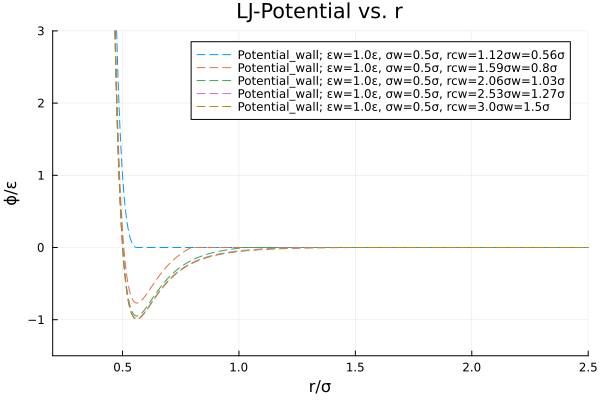
\includegraphics[width=\textwidth]{image/RaRtmap_LJ/LJ-Potential_Rt0.0.png}
      \subcaption{$\text{R}_\text{t}:0.0$}
      \label{}
    \end{minipage} &
    \begin{minipage}[t]{0.2\hsize}
      \centering
      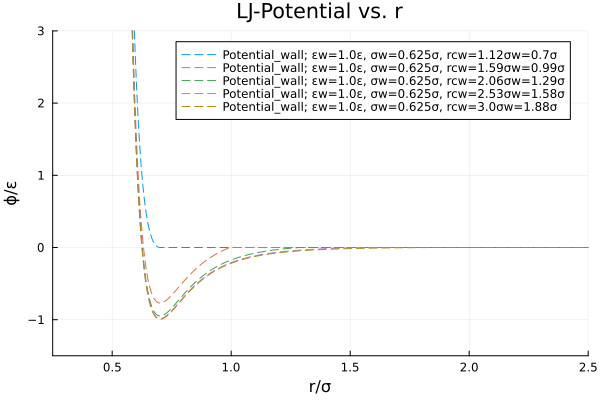
\includegraphics[width=\textwidth]{image/RaRtmap_LJ/LJ-Potential_Rt0.125.png}
      \subcaption{$\text{R}_\text{t}:0.125$}
      \label{}
    \end{minipage} &
    \begin{minipage}[t]{0.2\hsize}
      \centering
      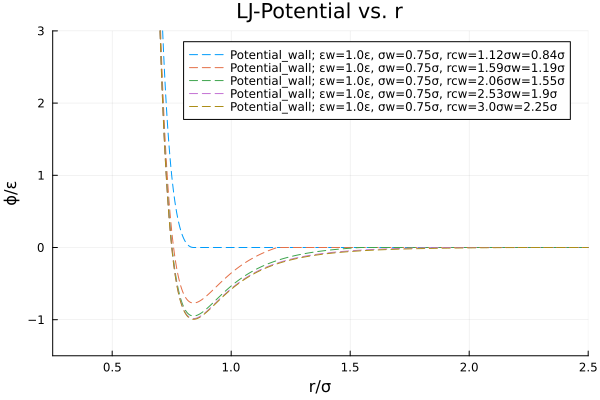
\includegraphics[width=\textwidth]{image/RaRtmap_LJ/LJ-Potential_Rt0.25.png}
      \subcaption{$\text{R}_\text{t}:0.25$}
      \label{}
    \end{minipage} &
    \begin{minipage}[t]{0.2\hsize}
      \centering
      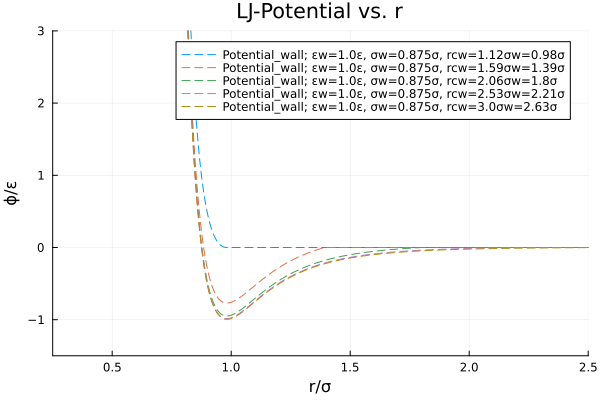
\includegraphics[width=\textwidth]{image/RaRtmap_LJ/LJ-Potential_Rt0.375.png}
      \subcaption{$\text{R}_\text{t}:0.375$}
      \label{}
    \end{minipage} &
    \begin{minipage}[t]{0.2\hsize}
      \centering
      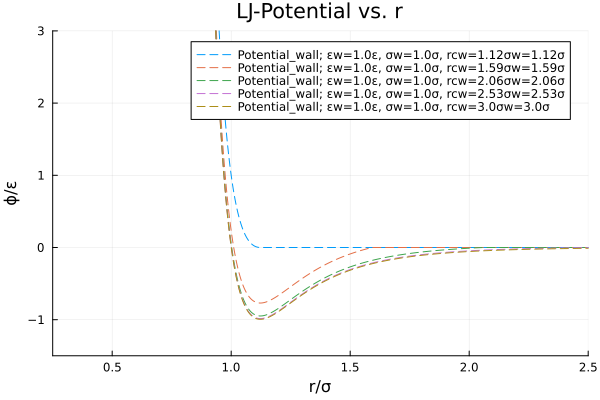
\includegraphics[width=\textwidth]{image/RaRtmap_LJ/LJ-Potential_Rt0.5.png}
      \subcaption{$\text{R}_\text{t}:0.5$}
      \label{}
    \end{minipage} 
  \end{tabular}
  \caption{LJ-potential}
  \label{}
\end{figure}

本章の以降の実験は特記がない限り以下のパラメータに近い値で行うものとする. 

\begin{itemize}
  \item $N = 1250$: 粒子数
  \item $\rho {\sigma}^2 = 0.4$: 粒子数密度
  \item $L_x / \sigma = 39.528471 \simeq 39.5$: 系の$x$幅
  \item $L_y / \sigma = 79.0569414 \simeq 79.0$: 系の$y$幅
  \item $k_{\text{B}} T / \varepsilon = 0.43$: 初期温度
  \item $k_{\text{B}} \Delta T / \varepsilon = 0.04$: 熱浴の温度差
  \item $mg\sigma/\varepsilon = 0.0003999718779659611 \simeq 4.0 \times 10^{-4}$: 粒子にかかる重力の大きさ
  \item $\dd t \sqrt{\epsilon/m{\sigma}^2} = 0.005$: シミュレーションにおける時間刻み.
\end{itemize}


以下に記すのは, 今後解析をする際に示すシミュレーションについての時間に関する説明である.

\begin{align}
  t_i &\colon シミュレーション開始時から, 物理量を解析する際にデータを採用し始める時間. これ以降は定常状態であるとみなす. \\
  t_f & \colon シミュレーション開始時から, シミュレーションの終了時までの時間.
\end{align}

いずれの実験の場合も$t\sqrt{\epsilon/m{\sigma}^2}=0$の時点では粒子は以下の画像のように, 系に規則正しく並べられているとする.

\begin{figure}[H]
  \centering
  
\includegraphics[scale=0.2]{image/initial1250.png}
  \caption{$N=1250$}
  \label{}
\end{figure}

\subsection{追実験}

壁を完全に濡らしている状態を考えたいので, $r^{\text{wall}}_{\text{cut}}=3.0\sigma$ に設定する.

また, 重力をかけた状態で粒子が下に落ちきり, 緩和しているとみなせるまでシミュレーションを行ってから, 熱流をかけている. この時点でのシミュレーションではデータを解析することはない.

\begin{itemize}
  \item $N = 5000$
  \item $\rho \sigma^2 = 0.4$
  \item $L_x / \sigma = 79.0\dots$
  \item $L_y / \sigma = 158.1\dots$
  \item $k_{\text{B}} T/\varepsilon = 4.3$
  \item $k_{\text{B}} \Delta T/\varepsilon = 0.0$
  \item $mg\sigma/\varepsilon = 2.0 \times 10^{-4}$
  \item $t_f \sqrt{\varepsilon / m \sigma^2} = 5.0 \times 10^{5}$
\end{itemize}

\begin{figure}[H]
  \centering
  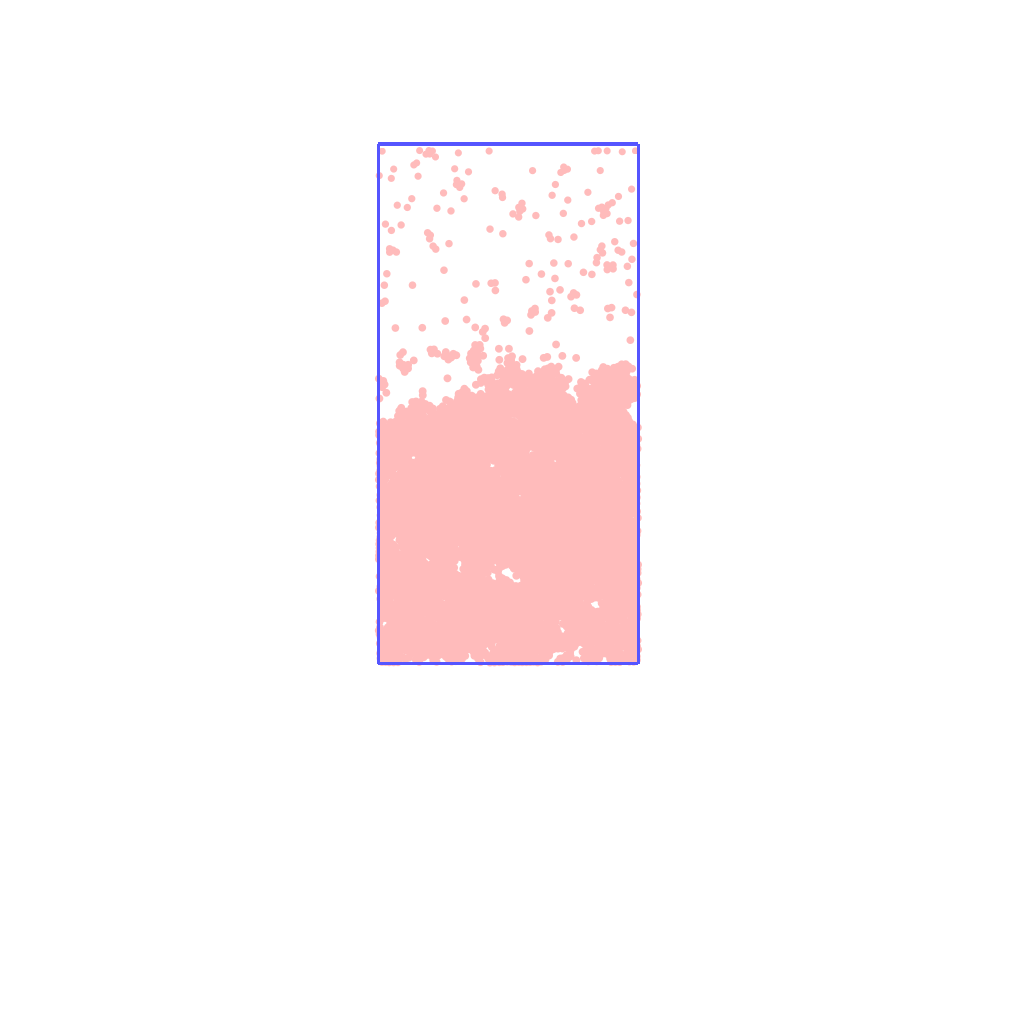
\includegraphics[scale=0.2]{image/drop5000.png}
  \caption{$t \sqrt{\varepsilon / m \sigma^2} = 5.0 \times 10^{5}$でのスナップショット}
  \label{}
\end{figure}

続いて重力をかけた緩和後の系で, 熱浴の温度差を改めて以下のようにつけ, 熱流をかけてシミュレーションをしている. このシミュレーションでデータを解析する.

\begin{itemize}
  \item $\chi = k_{\text{B}}\Delta T / mg L_y = 1.265$
  \item $k_{\text{B}} \Delta T/\varepsilon = 0.04$
  \item $t_i \sqrt{\varepsilon / m \sigma^2} = 5.0 \times 10^{5}$
  \item $t_f \sqrt{\varepsilon / m \sigma^2} = 1.0 \times 10^{6}$
\end{itemize}

$(\text{R}_\text{d} = 0.0, \text{R}_\text{t} = 0.5, \text{R}_\text{a} = 3.0 - 2^{1/6})$ で実験を行う. これは, $(\varepsilon^{\text{wall}} = \varepsilon, \sigma^{\text{wall}} = \sigma, r^{\text{wall}}_{\text{cut}} = 3.0 \sigma^{\text{wall}})$ に対応しているので, ${\phi_{\text{LJ}}}^{\text{wall}} = \phi_{\text{LJ}}$ ということになり, 先行研究と同じ結果を得ることができる.

\begin{figure}[H]
  \centering
  \href{https://youtu.be/CIEyUPvPY6A}{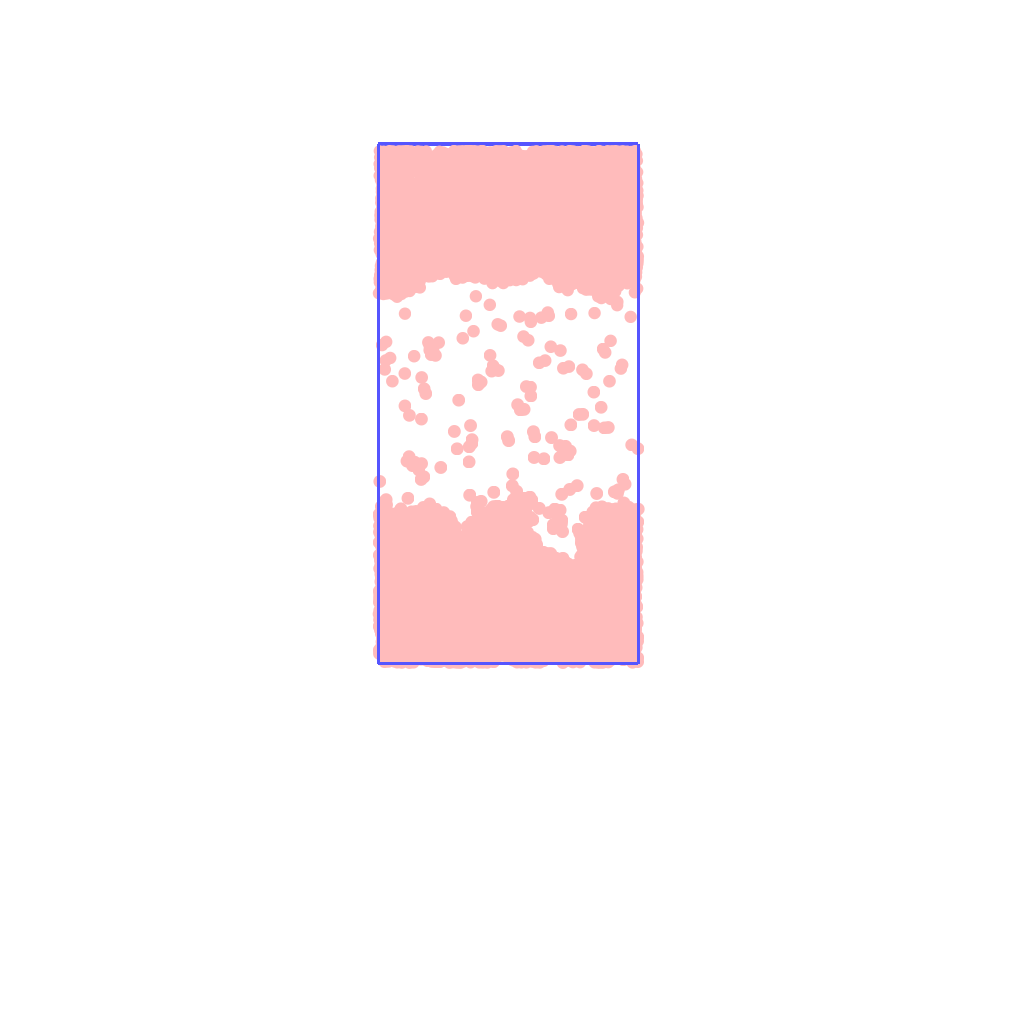
\includegraphics[scale=0.2]{image/2023-11-21T21:01:17.543_followup_chi1.265_Ay100_rho0.4_T0.43_dT0.04_Rd0.0_Rt0.5_Ra1.877538_g0.00019998593898298055_run1.0e8_output.png}}
  \caption{Ay100\_rho0.4\_T0.43\_dT0.04\_Rd0.0\_Rt0.5\_Ra1.877538\_g0.0004\_run1.0e8}
  \label{}
\end{figure}

\subsection{重力と熱流を同時にかける}

以下のように, $\text{R}_\text{a}$と$\text{R}_\text{t}$を少しずつ変えた系を設定して, それぞれシミュレーションをした.

\vspace{1\baselineskip}

\begin{tabular}{|c|c|c|c|c|c|} \hline
        & $\text{R}_\text{a}:0.0$ & $\text{R}_\text{a}:0.469$ & $\text{R}_\text{a}:0.938$ & $\text{R}_\text{a}:1.408$ & $\text{R}_\text{a}:1.877$ \\ \hline
  $\text{R}_\text{t}:0.0$ & a      & b      & c      & d      & e     \\ \hline
  $\text{R}_\text{t}:0.125$ & f      & g      & h      & i      & j     \\ \hline
  $\text{R}_\text{t}:0.25$ & k      & l      & m      & n      & o     \\ \hline
  $\text{R}_\text{t}:0.375$ & p      & q      & r      & s      & t     \\ \hline
  $\text{R}_\text{t}:0.5$ & u      & v      & w      & x      & y     \\ \hline
\end{tabular}

\vspace{1\baselineskip}

パラメータを確認する.

\begin{itemize}
  \item $N = 1250$
  \item $\rho {\sigma}^2 = 0.4$
  \item $L_x / \sigma = 39.5\dots$
  \item $L_y / \sigma = 79.0\dots$
  \item $k_{\text{B}} T / \varepsilon = 0.43$
  \item $k_{\text{B}} \Delta T / \varepsilon = 0.04$
  \item $mg\sigma/\varepsilon = 4.0 \times 10^{-4}$
  \item $t_f \sqrt{\varepsilon / m \sigma^2} = 2.0 \times 10^{5}$
\end{itemize}

この際の粒子集団の様相は以下のようになる.

\begin{figure}[H]
  \begin{tabular}{ccccc}
    \begin{minipage}[t]{0.2\hsize}
      \centering
      \href{https://youtu.be/yc-GeIQBuCk}{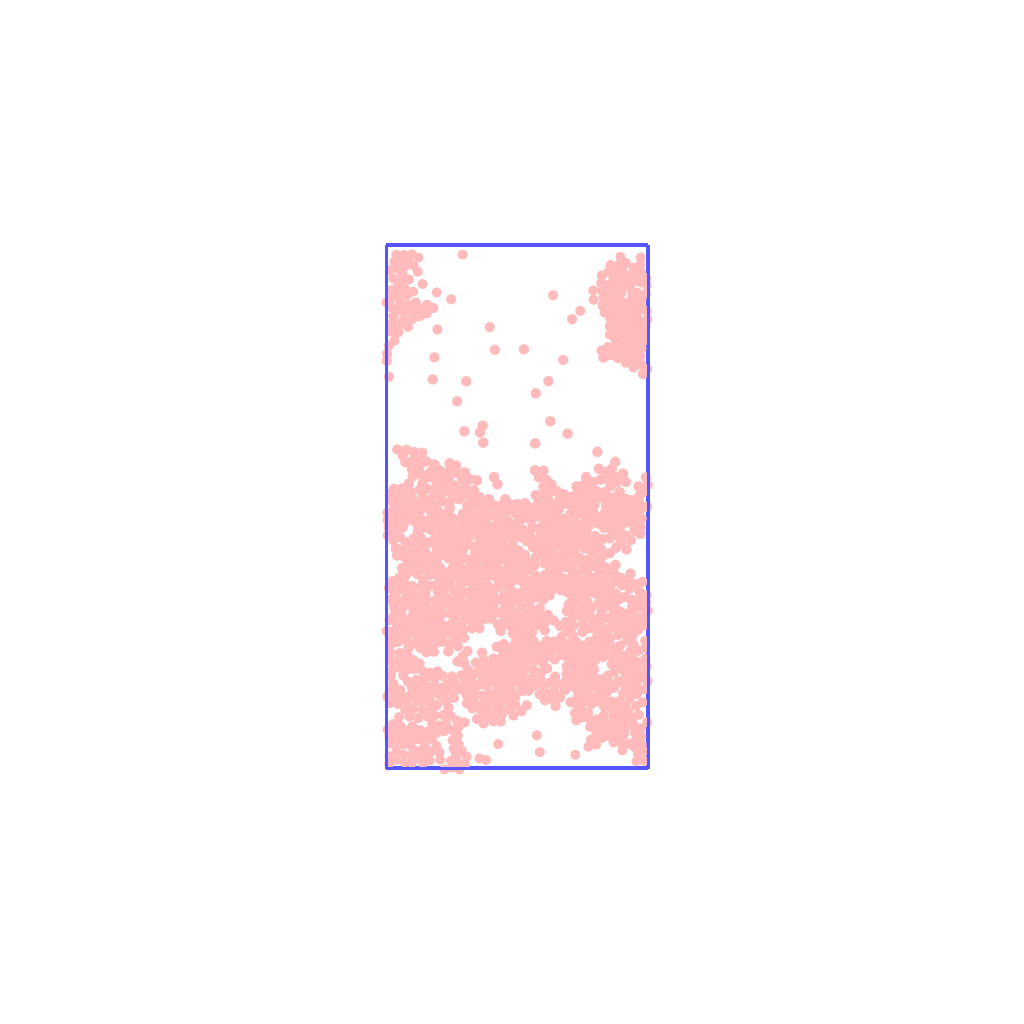
\includegraphics[width=\textwidth]{image/RaRtmap/2023-11-14T18:19:29.358__chi1.265_Ay50_rho0.4_T0.43_dT0.04_Rd0.0_Rt0.0_Ra0.0_g0.0003999718779659611_run4.0e7_output.png}}
      \subcaption{$\text{R}_\text{a}=0.0,\\\text{R}_\text{t}=0.0$}
      % \label{}
    \end{minipage} &
    \begin{minipage}[t]{0.2\hsize}
      \centering
      \href{https://youtu.be/4rNNLx9_DZ4}{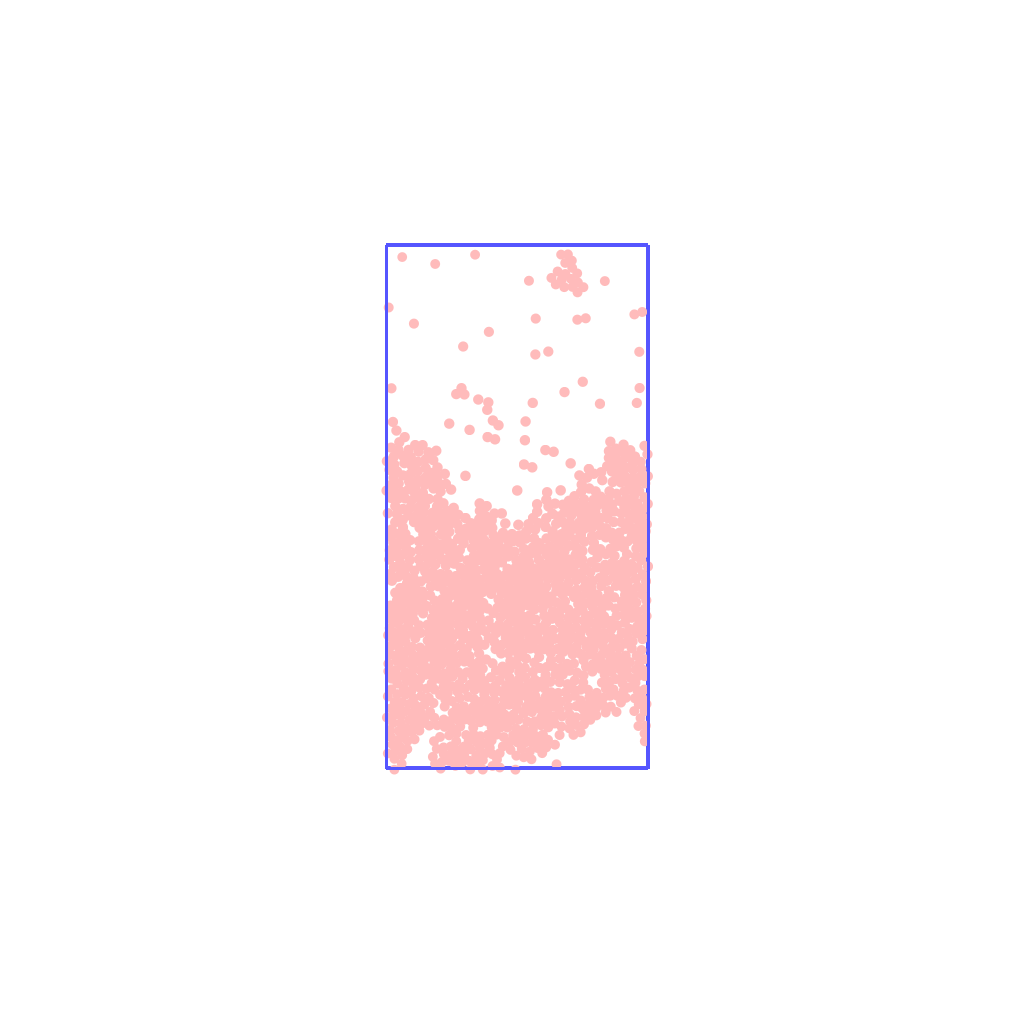
\includegraphics[width=\textwidth]{image/RaRtmap/2023-11-14T19:14:52.710__chi1.265_Ay50_rho0.4_T0.43_dT0.04_Rd0.0_Rt0.0_Ra0.4693845_g0.0003999718779659611_run4.0e7_output.png}}
      \subcaption{$\text{R}_\text{a}=0.469,\\\text{R}_\text{t}=0.0$}
      % \label{}
    \end{minipage} &
    \begin{minipage}[t]{0.2\hsize}
      \centering
      \href{https://youtu.be/QKLz7NzBte8}{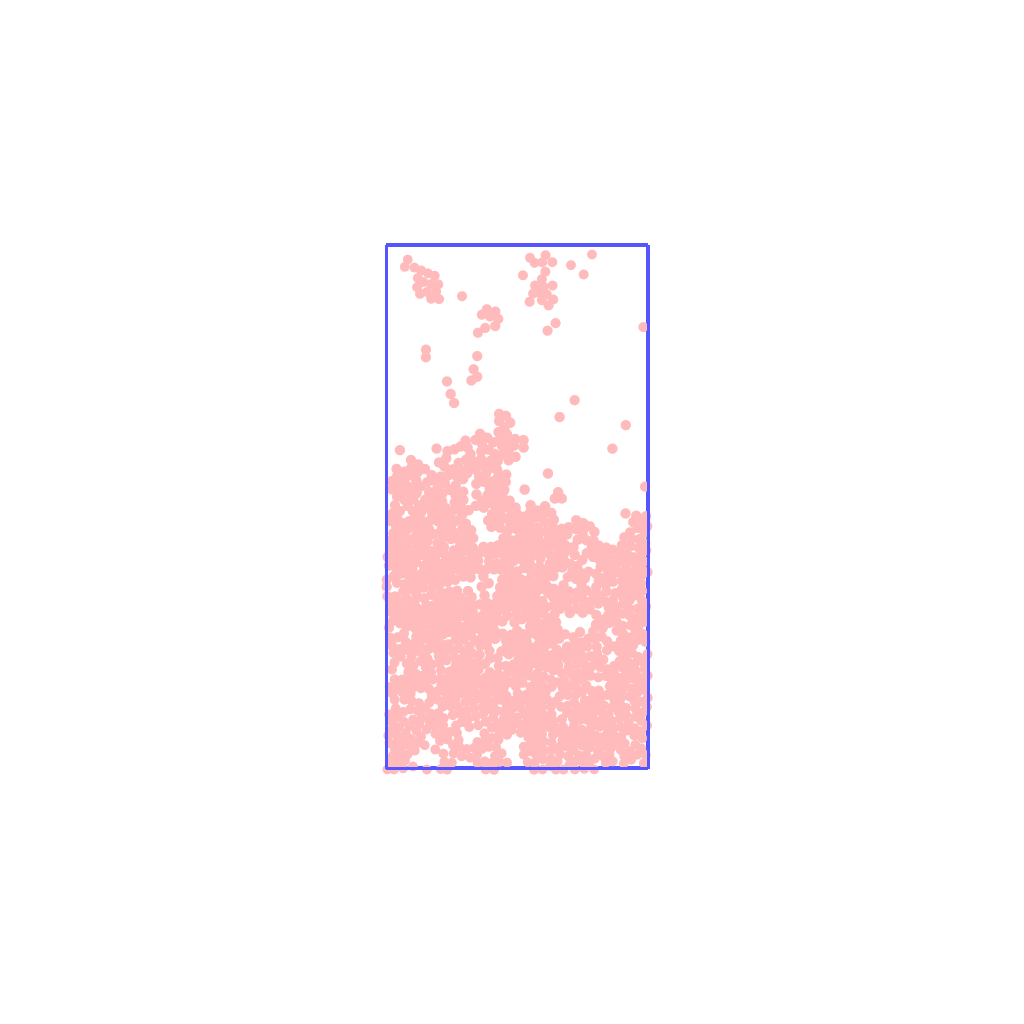
\includegraphics[width=\textwidth]{image/RaRtmap/2023-11-14T20:07:58.625__chi1.265_Ay50_rho0.4_T0.43_dT0.04_Rd0.0_Rt0.0_Ra0.938769_g0.0003999718779659611_run4.0e7_output.png}}
      \subcaption{$\text{R}_\text{a}=0.938,\\\text{R}_\text{t}=0.0$}
      % \label{}
    \end{minipage} &
    \begin{minipage}[t]{0.2\hsize}
      \centering
      \href{https://youtu.be/6iqcv_Af2U8}{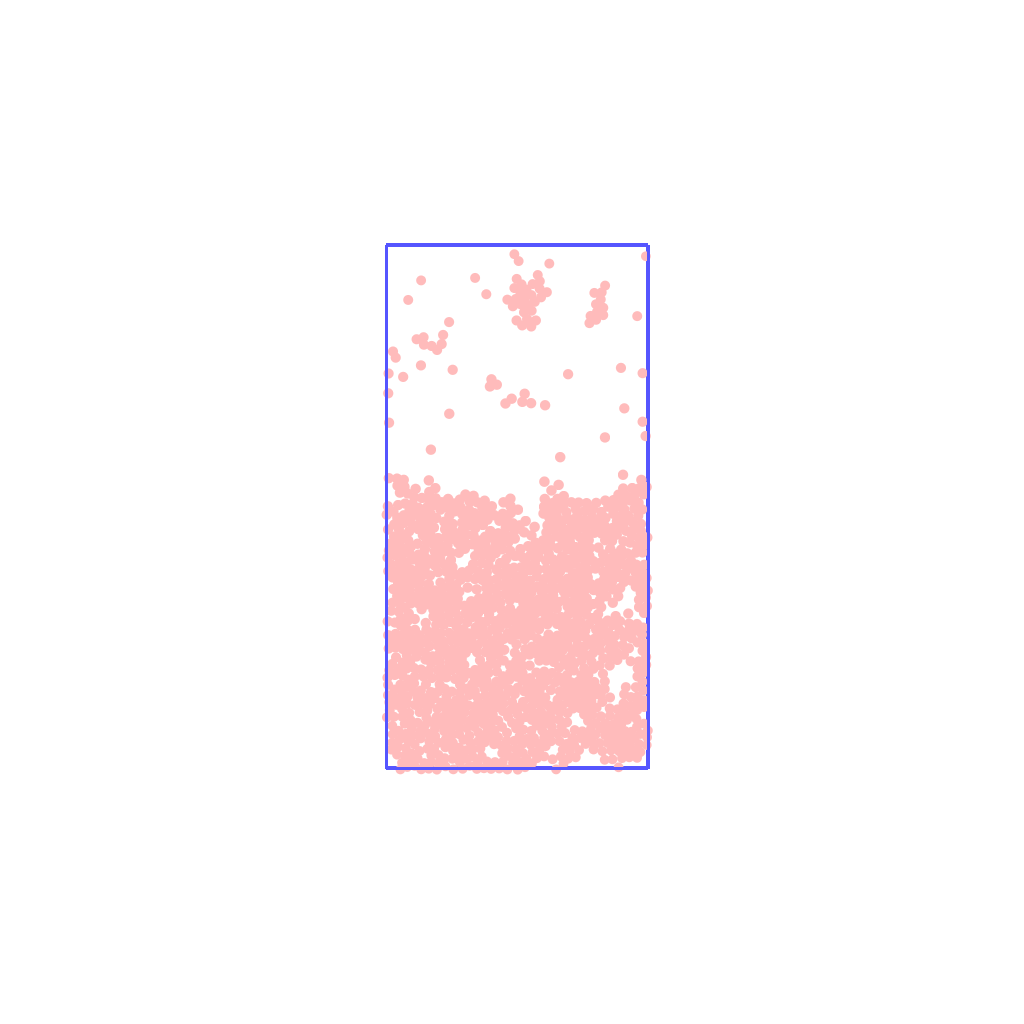
\includegraphics[width=\textwidth]{image/RaRtmap/2023-11-14T21:01:09.992__chi1.265_Ay50_rho0.4_T0.43_dT0.04_Rd0.0_Rt0.0_Ra1.4081535_g0.0003999718779659611_run4.0e7_output.png}}
      \subcaption{$\text{R}_\text{a}=1.408,\\\text{R}_\text{t}=0.0$}
      % \label{}
    \end{minipage} &
    \begin{minipage}[t]{0.2\hsize}
      \centering
      \href{https://youtu.be/Tn1Hd2eR0yo}{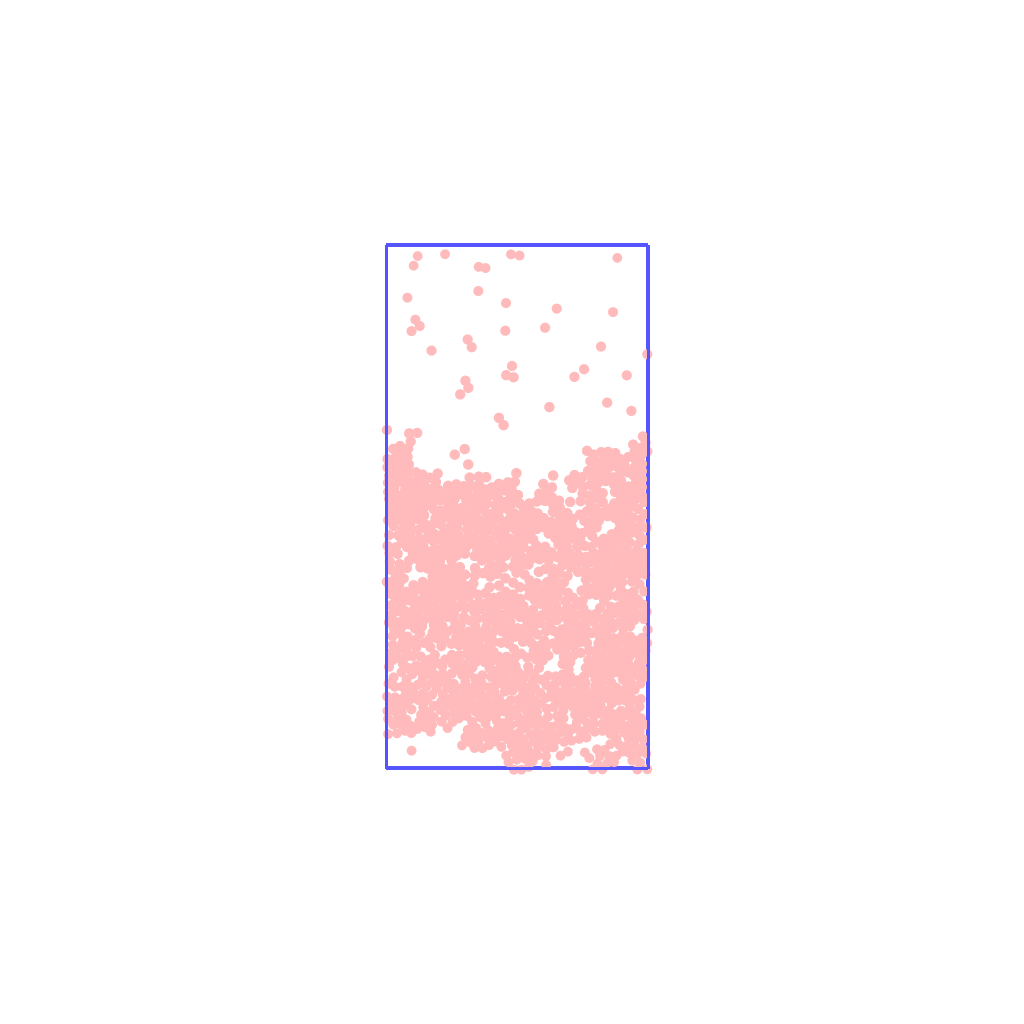
\includegraphics[width=\textwidth]{image/RaRtmap/2023-11-14T21:54:59.835__chi1.265_Ay50_rho0.4_T0.43_dT0.04_Rd0.0_Rt0.0_Ra1.877538_g0.0003999718779659611_run4.0e7_output.png}}
      \subcaption{$\text{R}_\text{a}=1.877,\\\text{R}_\text{t}=0.0$}
      % \label{}
    \end{minipage} \\
    \begin{minipage}[t]{0.2\hsize}
      \centering
      \href{https://youtu.be/B1GwQFCBszs}{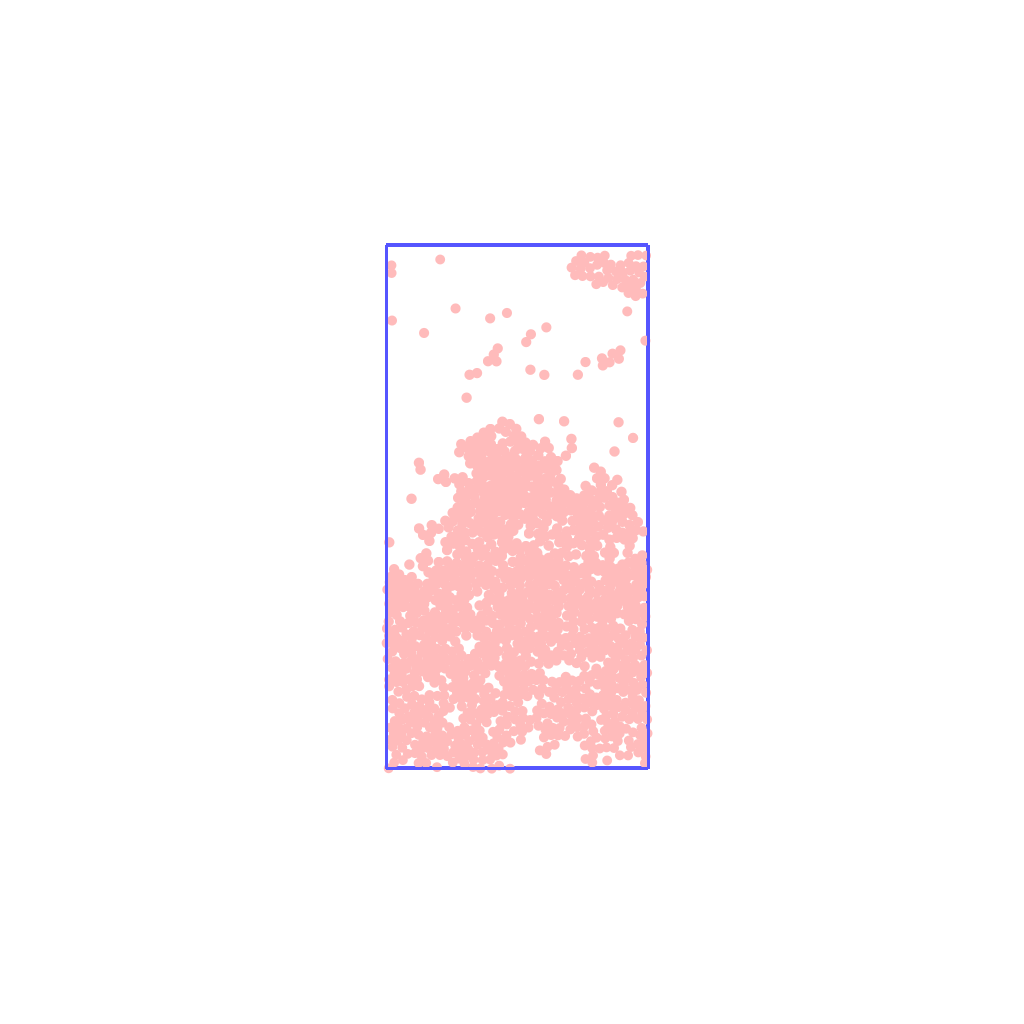
\includegraphics[width=\textwidth]{image/RaRtmap/2023-11-14T22:51:24.191__chi1.265_Ay50_rho0.4_T0.43_dT0.04_Rd0.0_Rt0.125_Ra0.0_g0.0003999718779659611_run4.0e7_output.png}}
      \subcaption{$\text{R}_\text{a}=0.0,\\\text{R}_\text{t}=0.125$}
      % \label{}
    \end{minipage} &
    \begin{minipage}[t]{0.2\hsize}
      \centering
      \href{https://youtu.be/MRIfAketXOI}{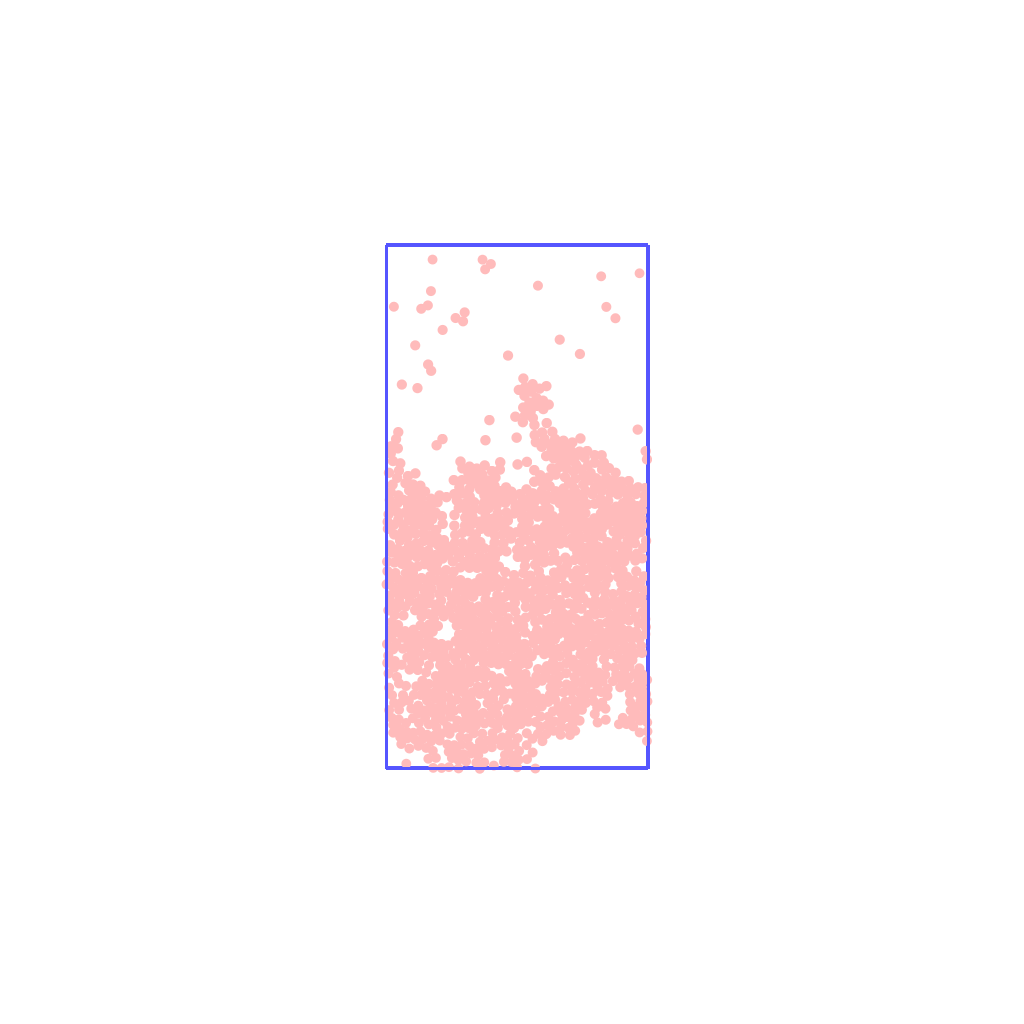
\includegraphics[width=\textwidth]{image/RaRtmap/2023-11-14T23:48:31.439__chi1.265_Ay50_rho0.4_T0.43_dT0.04_Rd0.0_Rt0.125_Ra0.4693845_g0.0003999718779659611_run4.0e7_output.png}}
      \subcaption{$\text{R}_\text{a}=0.469,\\\text{R}_\text{t}=0.125$}
      % \label{}
    \end{minipage} &
    \begin{minipage}[t]{0.2\hsize}
      \centering
      \href{https://youtu.be/v7rYxdoSSjI}{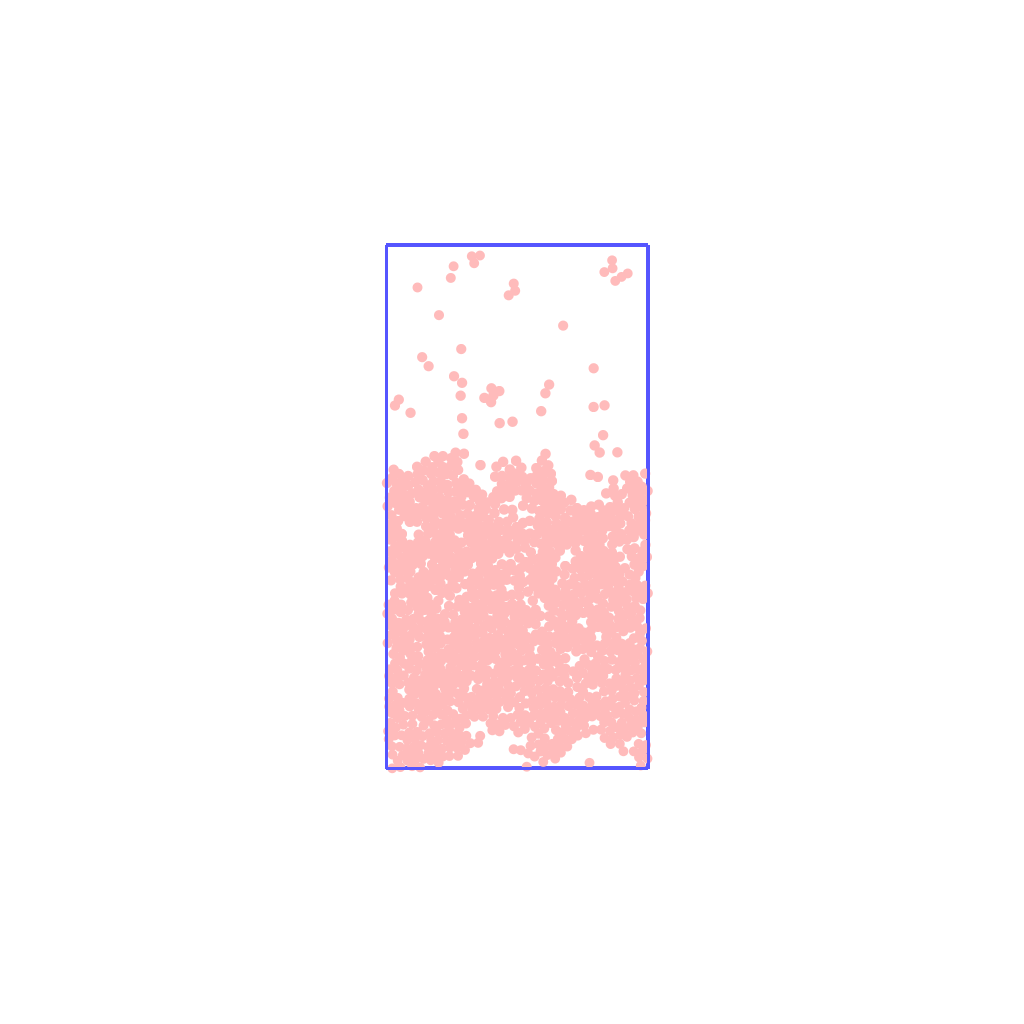
\includegraphics[width=\textwidth]{image/RaRtmap/2023-11-15T00:43:33.781__chi1.265_Ay50_rho0.4_T0.43_dT0.04_Rd0.0_Rt0.125_Ra0.938769_g0.0003999718779659611_run4.0e7_output.png}}
      \subcaption{$\text{R}_\text{a}=0.938,\\\text{R}_\text{t}=0.125$}
      % \label{}
    \end{minipage} &
    \begin{minipage}[t]{0.2\hsize}
      \centering
      \href{https://youtu.be/0NFYPFYBcc4}{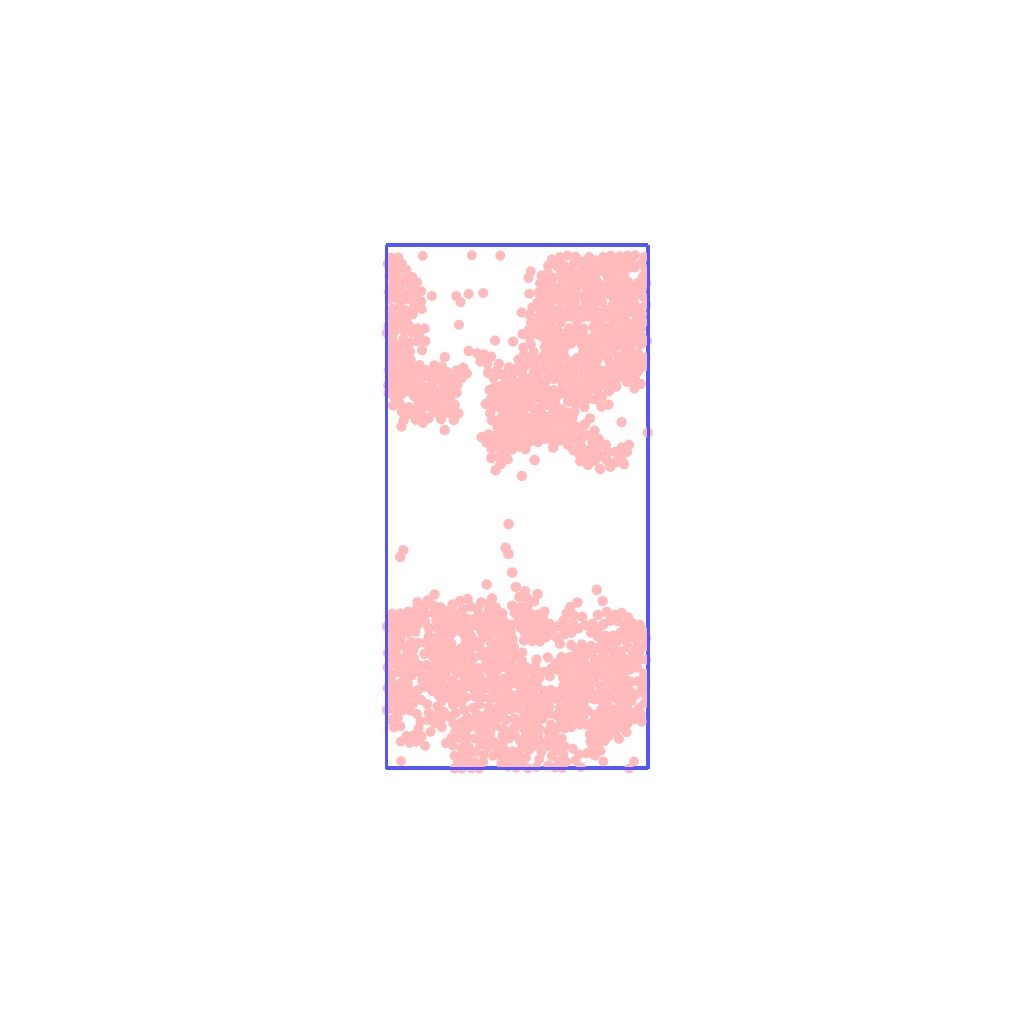
\includegraphics[width=\textwidth]{image/RaRtmap/2023-11-15T01:35:17.404__chi1.265_Ay50_rho0.4_T0.43_dT0.04_Rd0.0_Rt0.125_Ra1.4081535_g0.0003999718779659611_run4.0e7_output.png}}
      \subcaption{$\text{R}_\text{a}=1.408,\\\text{R}_\text{t}=0.125$}
      % \label{}
    \end{minipage} &
    \begin{minipage}[t]{0.2\hsize}
      \centering
      \href{https://youtu.be/FXTDOcpARl0}{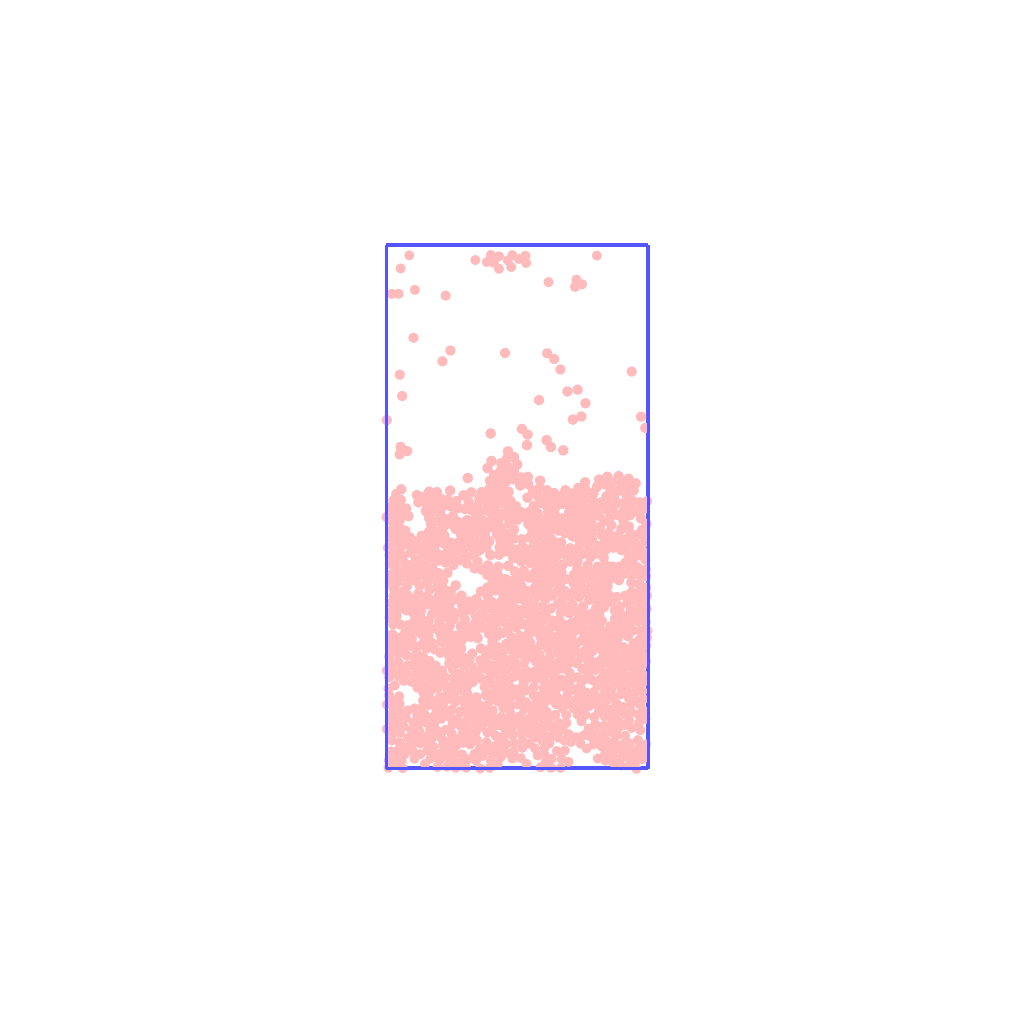
\includegraphics[width=\textwidth]{image/RaRtmap/2023-11-15T02:27:34.337__chi1.265_Ay50_rho0.4_T0.43_dT0.04_Rd0.0_Rt0.125_Ra1.877538_g0.0003999718779659611_run4.0e7_output.png}}
      \subcaption{$\text{R}_\text{a}=1.877,\\\text{R}_\text{t}=0.125$}
      % \label{}
    \end{minipage} \\
    \begin{minipage}[t]{0.2\hsize}
      \centering
      \href{https://youtu.be/4A\_MHNHZrKQ}{
      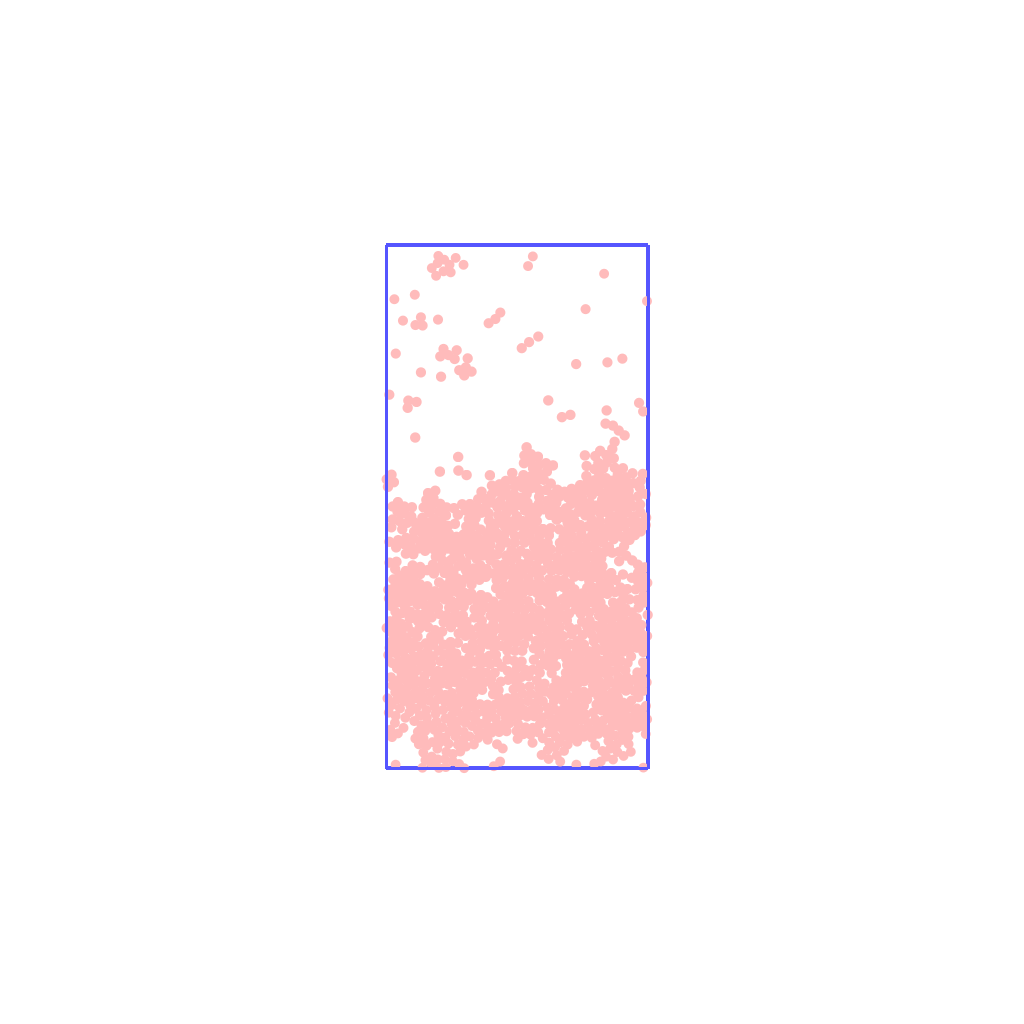
\includegraphics[width=\textwidth]{image/RaRtmap/2023-11-15T03:19:32.715__chi1.265_Ay50_rho0.4_T0.43_dT0.04_Rd0.0_Rt0.25_Ra0.0_g0.0003999718779659611_run4.0e7_output.png}}
      \subcaption{$\text{R}_\text{a}=0.0,\\\text{R}_\text{t}=0.250$}
      % \label{}
    \end{minipage} &
    \begin{minipage}[t]{0.2\hsize}
      \centering
      \href{https://youtu.be/jGzUPm\_3oH0}{
      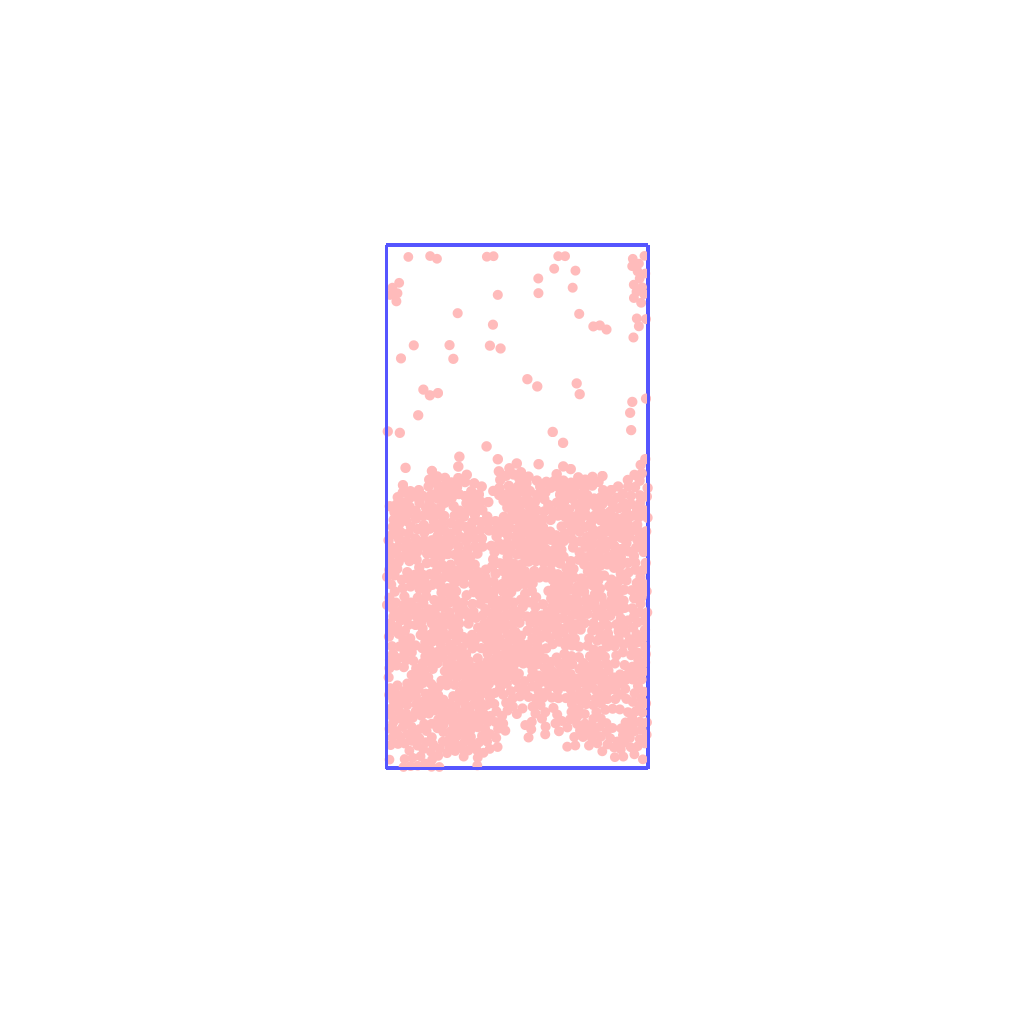
\includegraphics[width=\textwidth]{image/RaRtmap/2023-11-15T04:11:00.956__chi1.265_Ay50_rho0.4_T0.43_dT0.04_Rd0.0_Rt0.25_Ra0.4693845_g0.0003999718779659611_run4.0e7_output.png}}
      \subcaption{$\text{R}_\text{a}=0.469,\\\text{R}_\text{t}=0.250$}
      % \label{}
    \end{minipage} &
    \begin{minipage}[t]{0.2\hsize}
      \centering
      \href{https://youtu.be/0iyDEBwDF7A}{
      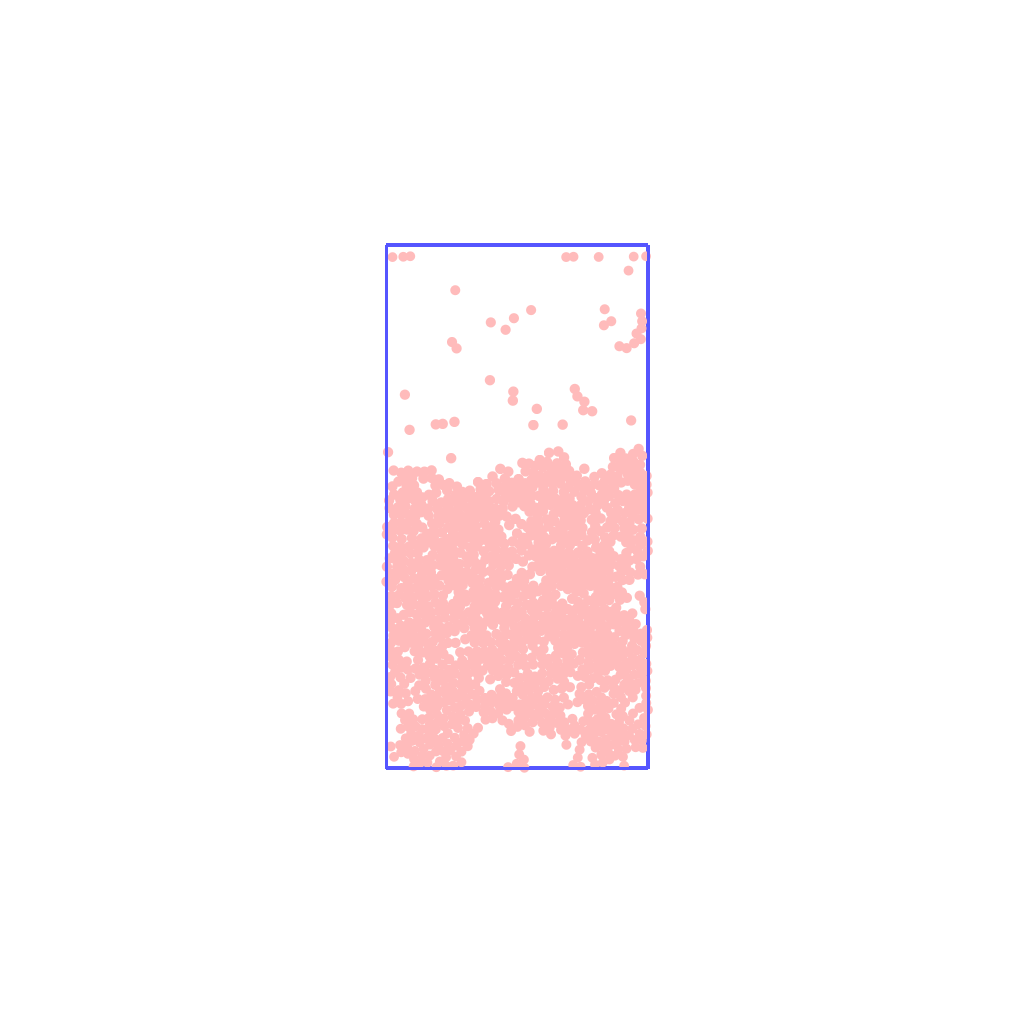
\includegraphics[width=\textwidth]{image/RaRtmap/2023-11-15T05:03:45.973__chi1.265_Ay50_rho0.4_T0.43_dT0.04_Rd0.0_Rt0.25_Ra0.938769_g0.0003999718779659611_run4.0e7_output.png}}
      \subcaption{$\text{R}_\text{a}=0.938,\\\text{R}_\text{t}=0.250$}
      % \label{}
    \end{minipage} &
    \begin{minipage}[t]{0.2\hsize}
      \centering
      \href{https://youtu.be/Sqk3HDSDINw}{
      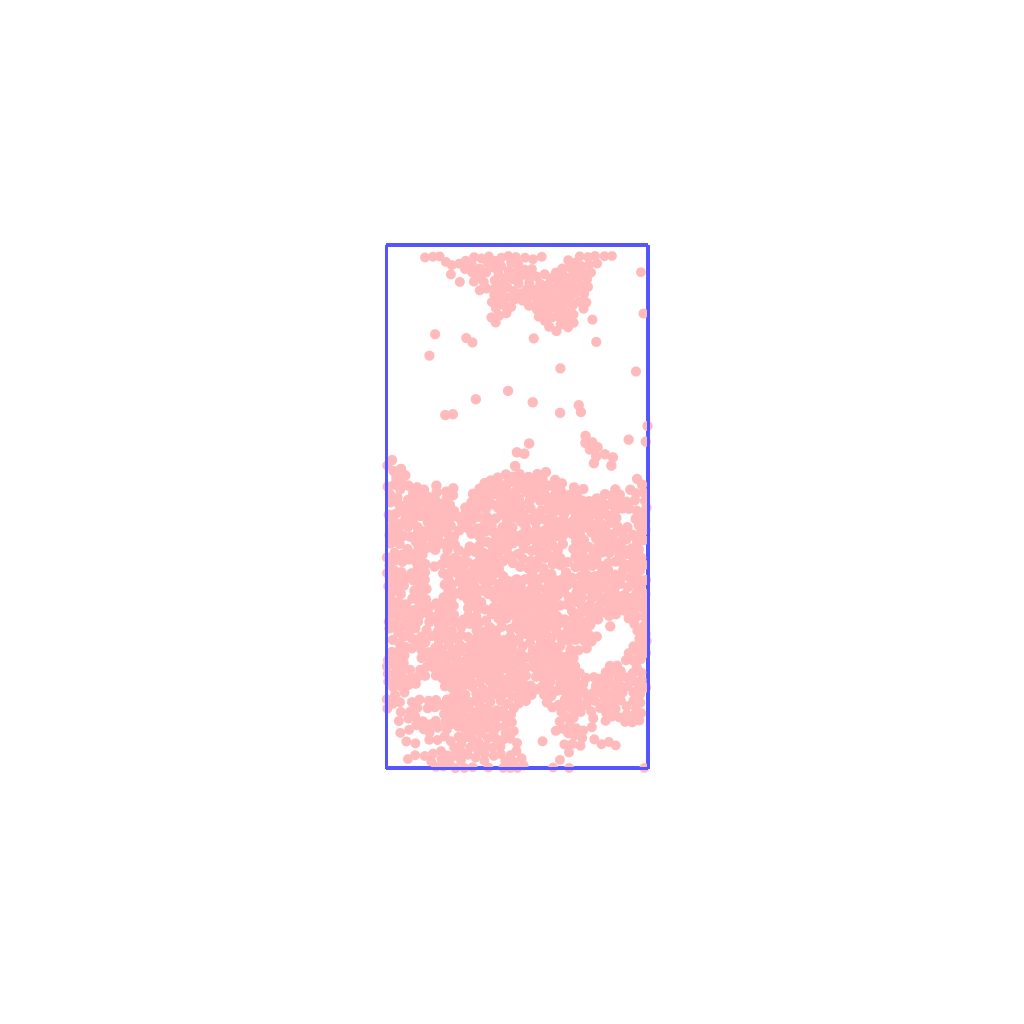
\includegraphics[width=\textwidth]{image/RaRtmap/2023-11-15T05:53:00.667__chi1.265_Ay50_rho0.4_T0.43_dT0.04_Rd0.0_Rt0.25_Ra1.4081535_g0.0003999718779659611_run4.0e7_output.png}}
      \subcaption{$\text{R}_\text{a}=1.408,\\\text{R}_\text{t}=0.250$}
      % \label{}
    \end{minipage} &
    \begin{minipage}[t]{0.2\hsize}
      \centering
      \href{https://youtu.be/3lqCLQchVYA}{
      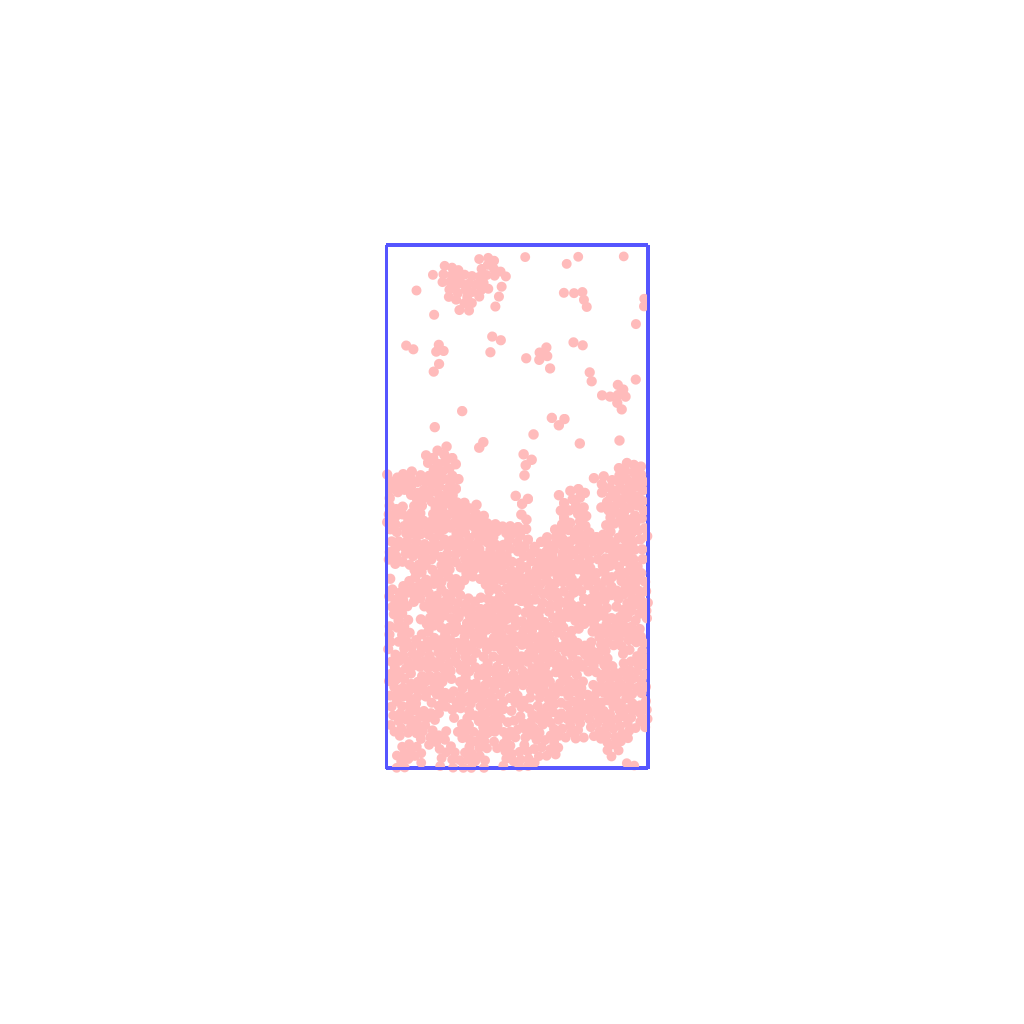
\includegraphics[width=\textwidth]{image/RaRtmap/2023-11-15T06:43:21.554__chi1.265_Ay50_rho0.4_T0.43_dT0.04_Rd0.0_Rt0.25_Ra1.877538_g0.0003999718779659611_run4.0e7_output.png}}
      \subcaption{$\text{R}_\text{a}=1.877,\\\text{R}_\text{t}=0.250$}
      % \label{}
    \end{minipage} \\
    \begin{minipage}[t]{0.2\hsize}
      \centering
      \href{https://youtu.be/1cMmZVmcThA}{
      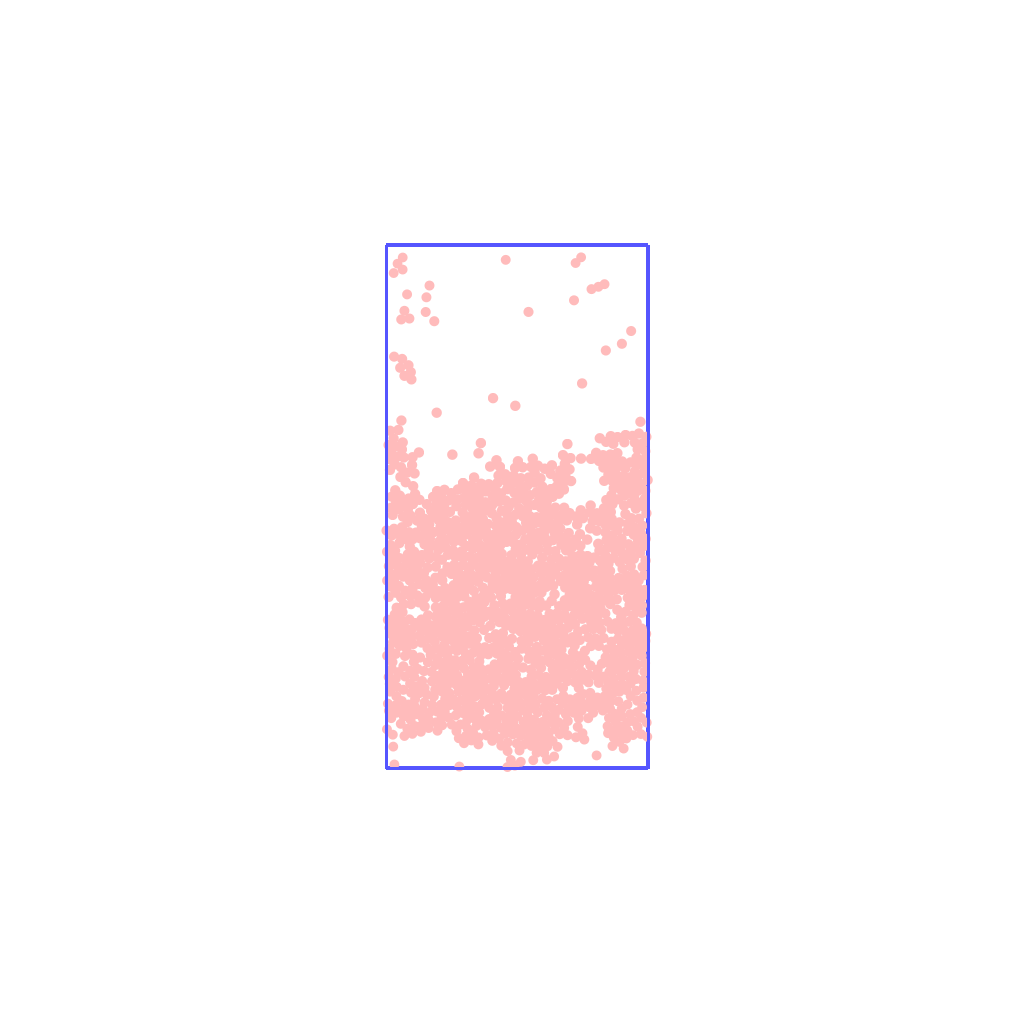
\includegraphics[width=\textwidth]{image/RaRtmap/2023-11-15T07:34:00.555__chi1.265_Ay50_rho0.4_T0.43_dT0.04_Rd0.0_Rt0.375_Ra0.0_g0.0003999718779659611_run4.0e7_output.png}}
      \subcaption{$\text{R}_\text{a}=0.0,\\\text{R}_\text{t}=0.375$}
      % \label{}
    \end{minipage} &
    \begin{minipage}[t]{0.2\hsize}
      \centering
      \href{https://youtu.be/MDWWS7Axo-4}{
      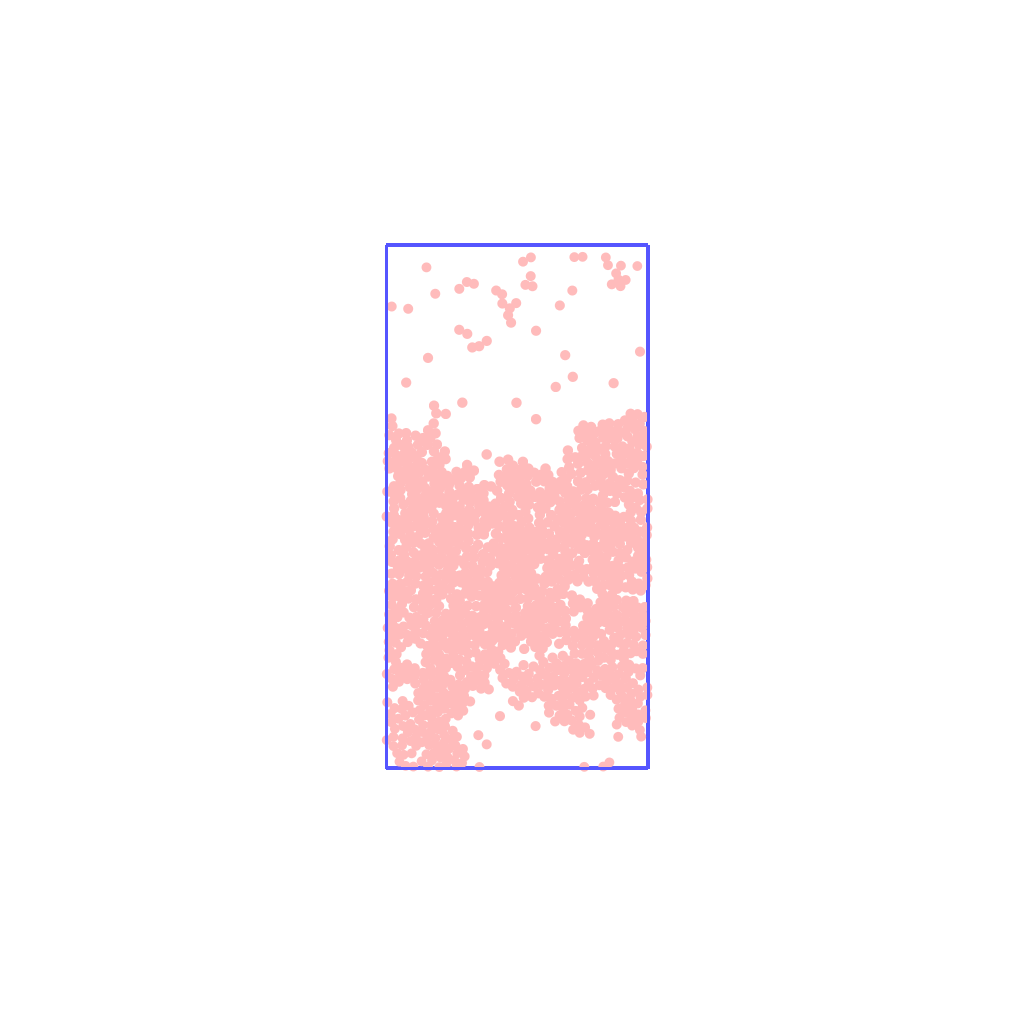
\includegraphics[width=\textwidth]{image/RaRtmap/2023-11-15T08:24:37.362__chi1.265_Ay50_rho0.4_T0.43_dT0.04_Rd0.0_Rt0.375_Ra0.4693845_g0.0003999718779659611_run4.0e7_output.png}}
      \subcaption{$\text{R}_\text{a}=0.469,\\\text{R}_\text{t}=0.375$}
      % \label{}
    \end{minipage} &
    \begin{minipage}[t]{0.2\hsize}
      \centering
      \href{https://youtu.be/Y6O_tVs6mHY}{
      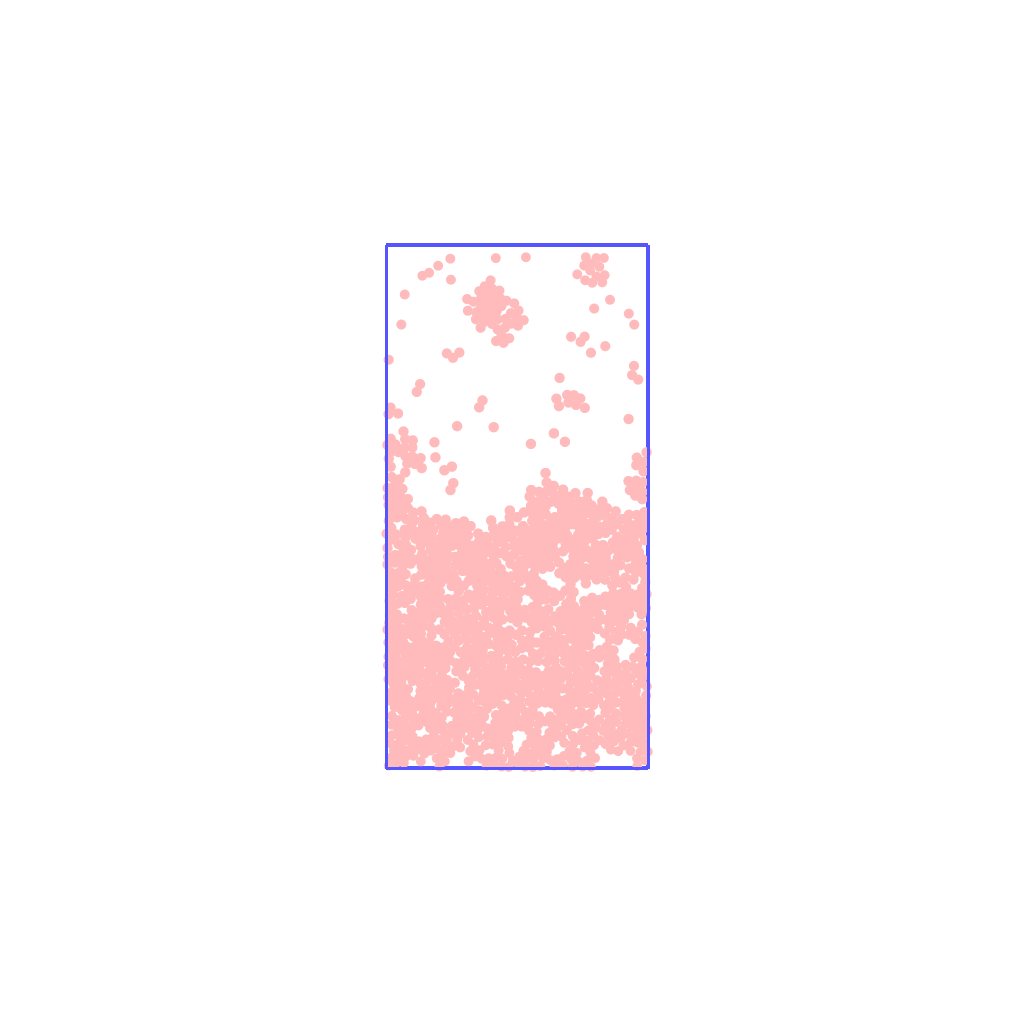
\includegraphics[width=\textwidth]{image/RaRtmap/2023-11-15T09:16:40.082__chi1.265_Ay50_rho0.4_T0.43_dT0.04_Rd0.0_Rt0.375_Ra0.938769_g0.0003999718779659611_run4.0e7_output.png}}
      \subcaption{$\text{R}_\text{a}=0.938,\\\text{R}_\text{t}=0.375$}
      % \label{}
    \end{minipage} &
    \begin{minipage}[t]{0.2\hsize}
      \centering
      \href{https://youtu.be/yeI5CDT0TEw}{
      
\includegraphics[width=\textwidth]{image/RaRtmap/2023-11-15T10:07:20.945__chi1.265_Ay50_rho0.4_T0.43_dT0.04_Rd0.0_Rt0.375_Ra1.4081535_g0.0003999718779659611_run4.0e7_output.png}}
      \subcaption{$\text{R}_\text{a}=1.408,\\\text{R}_\text{t}=0.375$}
      % \label{}
    \end{minipage} &
    \begin{minipage}[t]{0.2\hsize}
      \centering
      \href{https://youtu.be/h6w-DYqP-bg}{
      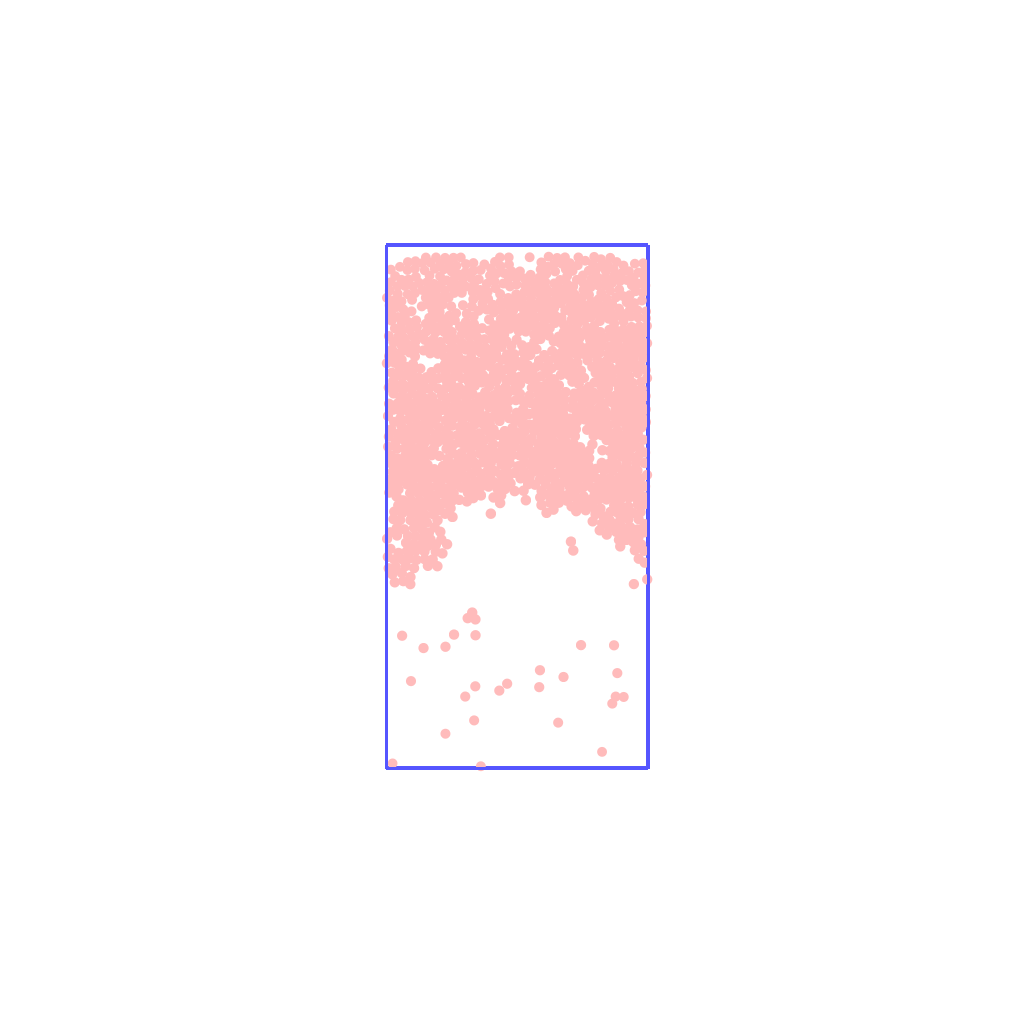
\includegraphics[width=\textwidth]{image/RaRtmap/2023-11-15T10:59:30.665__chi1.265_Ay50_rho0.4_T0.43_dT0.04_Rd0.0_Rt0.375_Ra1.877538_g0.0003999718779659611_run4.0e7_output.png}}
      \subcaption{$\text{R}_\text{a}=1.877,\\\text{R}_\text{t}=0.375$}
      % \label{}
    \end{minipage} \\
    \begin{minipage}[t]{0.2\hsize}
      \centering
      \href{https://youtu.be/S0NOYiYNCBU}{
      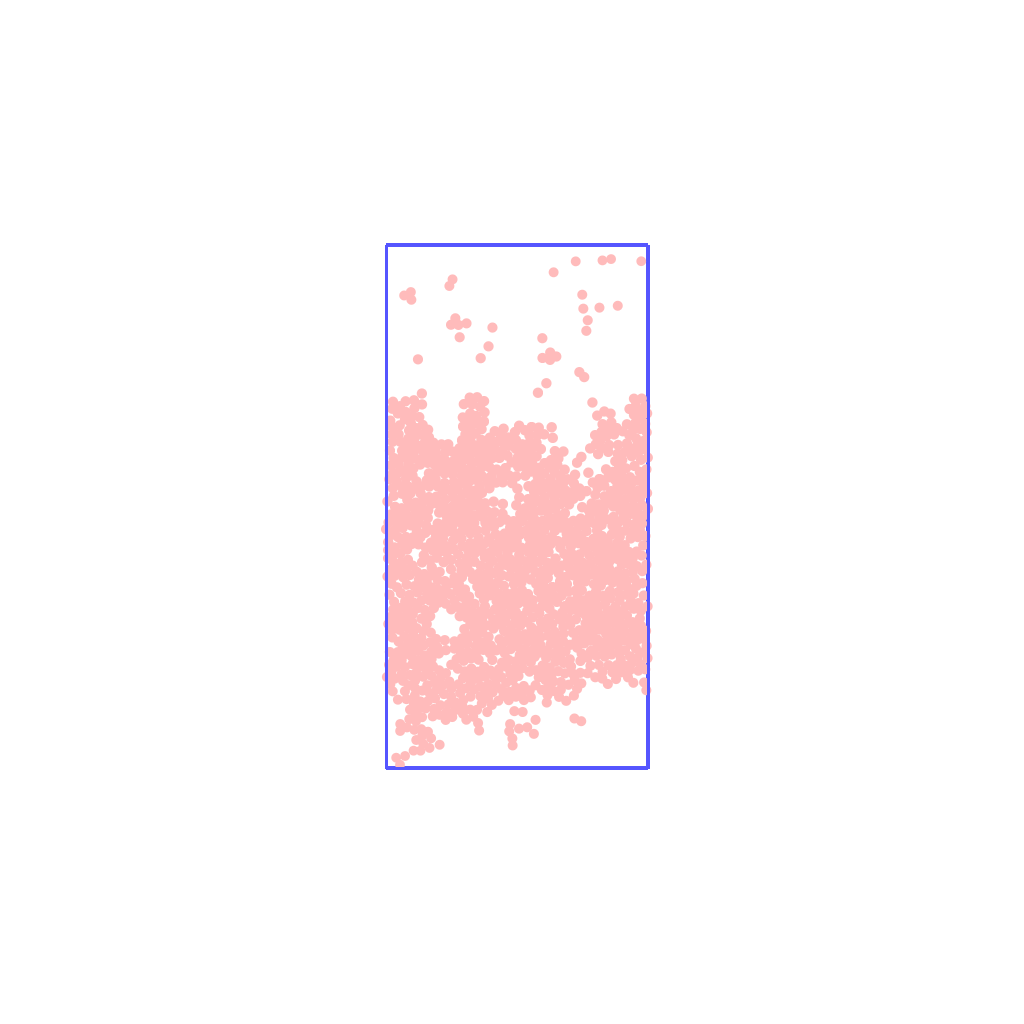
\includegraphics[width=\textwidth]{image/RaRtmap/2023-11-15T11:53:37.697__chi1.265_Ay50_rho0.4_T0.43_dT0.04_Rd0.0_Rt0.5_Ra0.0_g0.0003999718779659611_run4.0e7_output.png}}
      \subcaption{$\text{R}_\text{a}=0.0,\\\text{R}_\text{t}=0.500$}
      % \label{}
    \end{minipage} &
    \begin{minipage}[t]{0.2\hsize}
      \centering
      \href{https://youtu.be/l8Mz0kOFZwY}{
      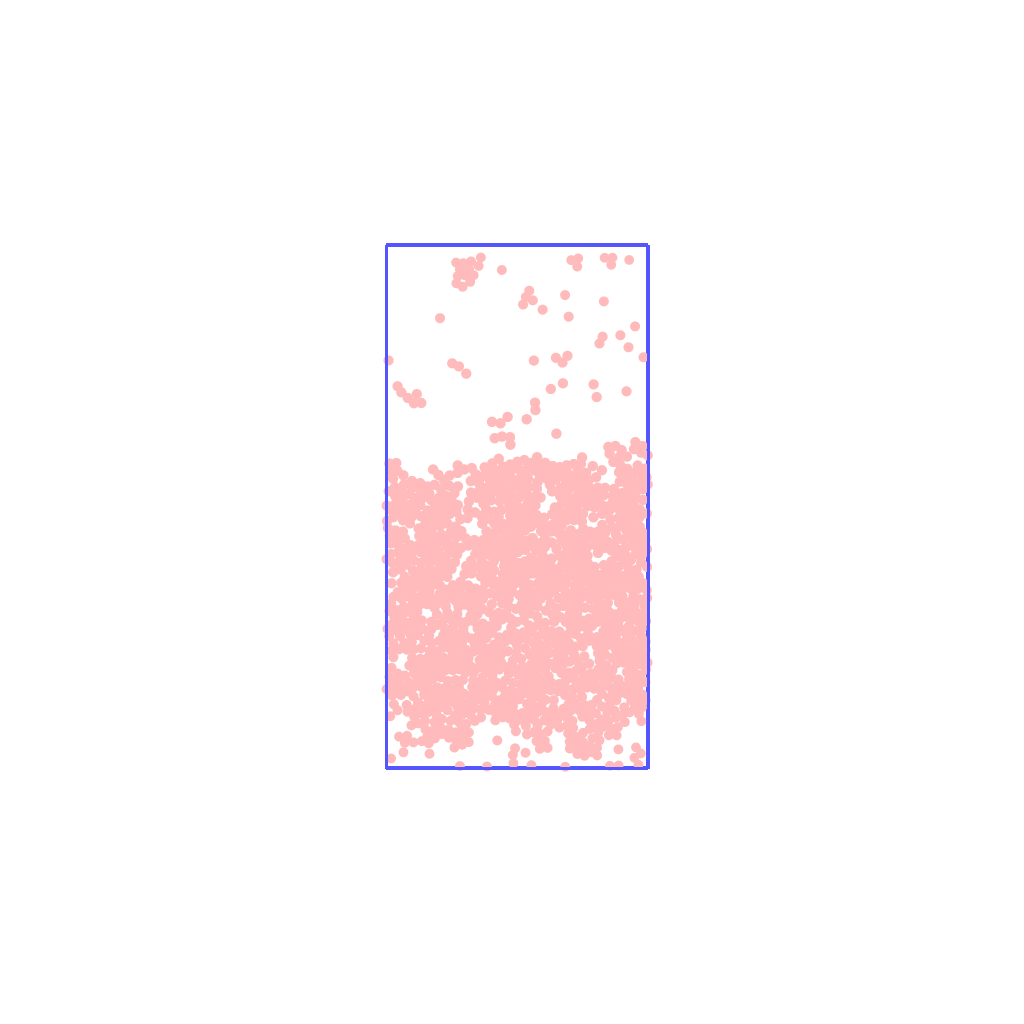
\includegraphics[width=\textwidth]{image/RaRtmap/2023-11-15T12:45:26.303__chi1.265_Ay50_rho0.4_T0.43_dT0.04_Rd0.0_Rt0.5_Ra0.4693845_g0.0003999718779659611_run4.0e7_output.png}}
      \subcaption{$\text{R}_\text{a}=0.469,\\\text{R}_\text{t}=0.500$}
      % \label{}
    \end{minipage} &
    \begin{minipage}[t]{0.2\hsize}
      \centering
      \href{https://youtu.be/pR-P4R70FQg}{
      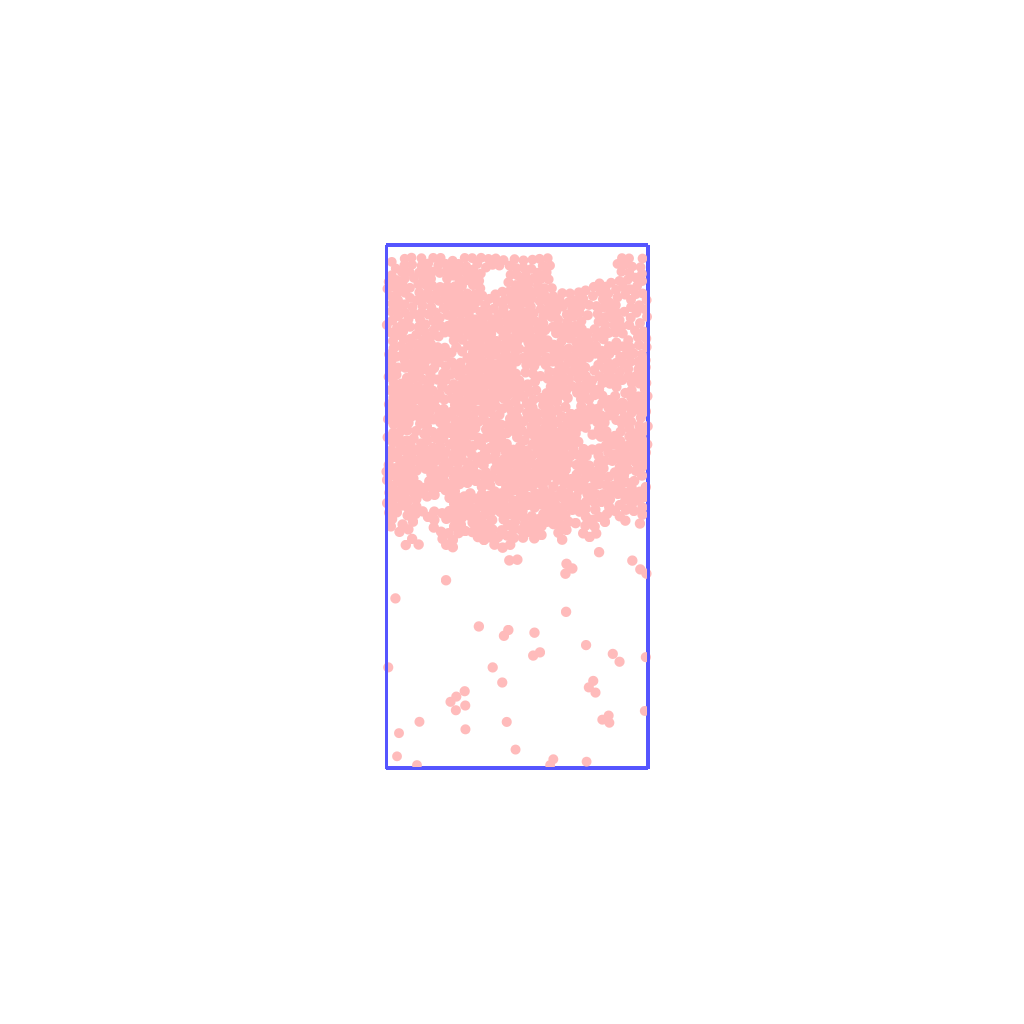
\includegraphics[width=\textwidth]{image/RaRtmap/2023-11-15T13:37:58.058__chi1.265_Ay50_rho0.4_T0.43_dT0.04_Rd0.0_Rt0.5_Ra0.938769_g0.0003999718779659611_run4.0e7_output.png}}
      \subcaption{$\text{R}_\text{a}=0.938,\\\text{R}_\text{t}=0.500$}
      % \label{}
    \end{minipage} &
    \begin{minipage}[t]{0.2\hsize}
      \centering
      \href{https://youtu.be/kSUk1XcKZBA}{
      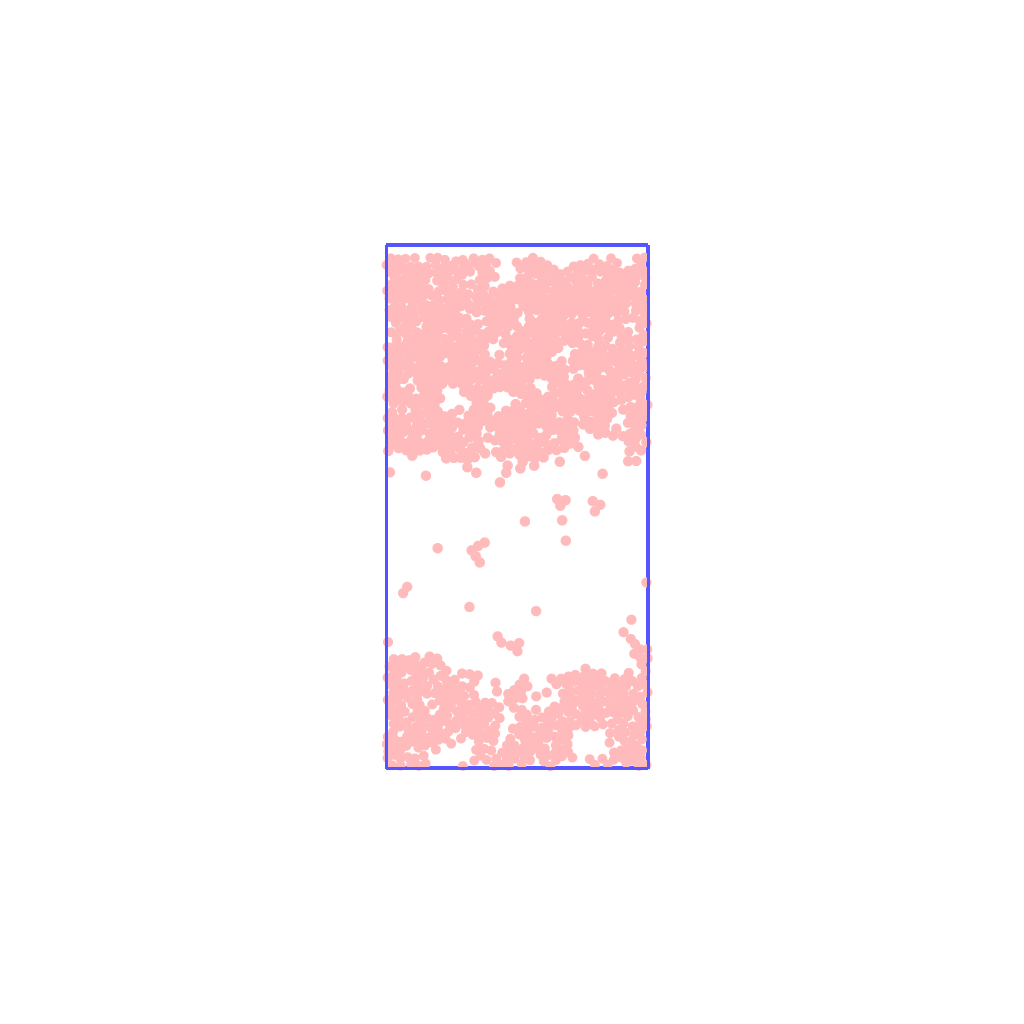
\includegraphics[width=\textwidth]{image/RaRtmap/2023-11-15T14:30:22.529__chi1.265_Ay50_rho0.4_T0.43_dT0.04_Rd0.0_Rt0.5_Ra1.4081535_g0.0003999718779659611_run4.0e7_output.png}}
      \subcaption{$\text{R}_\text{a}=1.408,\\\text{R}_\text{t}=0.500$}
      % \label{}
    \end{minipage} &
    \begin{minipage}[t]{0.2\hsize}
      \centering
      
\includegraphics[width=\textwidth]{image/RaRtmap/2023-11-15T15:21:59.073__chi1.265_Ay50_rho0.4_T0.43_dT0.04_Rd0.0_Rt0.5_Ra1.877538_g0.0003999718779659611_run4.0e7_output.png}
      \subcaption{$\text{R}_\text{a}=1.877,\\\text{R}_\text{t}=0.500$}
      % \label{}
    \end{minipage} 
  \end{tabular}
  \caption{}
  % \lable{}
\end{figure}


重心位置$Y_g$を系の$y$幅でスケーリングして, 時系列プロットすると,

\begin{align}
  Y_g &\equiv \bar{y_i} = \frac{1}{N} \sum_{i}^{N} y_i
\end{align}

\begin{figure}[H]
  \begin{tabular}{ccccc}
    \begin{minipage}[t]{0.2\hsize}
      \centering
      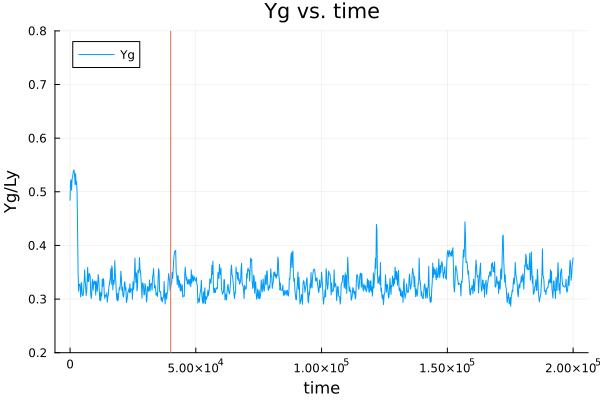
\includegraphics[width=\textwidth]{image/RaRtmap_time/2023-11-14T18:19:29.358__chi1.265_Ay50_rho0.4_T0.43_dT0.04_Rd0.0_Rt0.0_Ra0.0_g0.0003999718779659611_run4.0e7_output.png}
      \subcaption{$\text{R}_\text{a}=0.0,\\\text{R}_\text{t}=0.0$}
      \label{fig:RaRtmap_time_Ra0.0_Rt0.0}
    \end{minipage} &
    \begin{minipage}[t]{0.2\hsize}
      \centering
      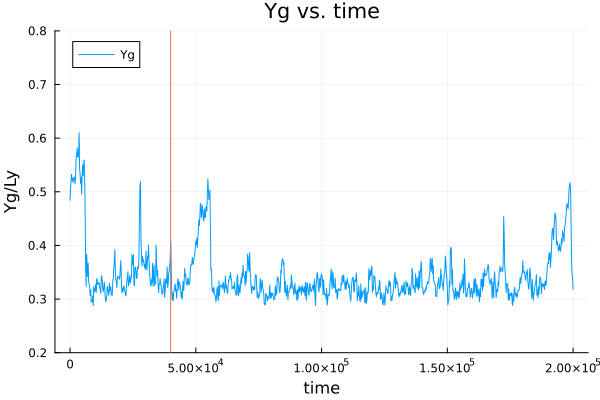
\includegraphics[width=\textwidth]{image/RaRtmap_time/2023-11-14T19:14:52.710__chi1.265_Ay50_rho0.4_T0.43_dT0.04_Rd0.0_Rt0.0_Ra0.4693845_g0.0003999718779659611_run4.0e7_output.png}
      \subcaption{$\text{R}_\text{a}=0.469,\\\text{R}_\text{t}=0.0$}
      \label{}
    \end{minipage} &
    \begin{minipage}[t]{0.2\hsize}
      \centering
      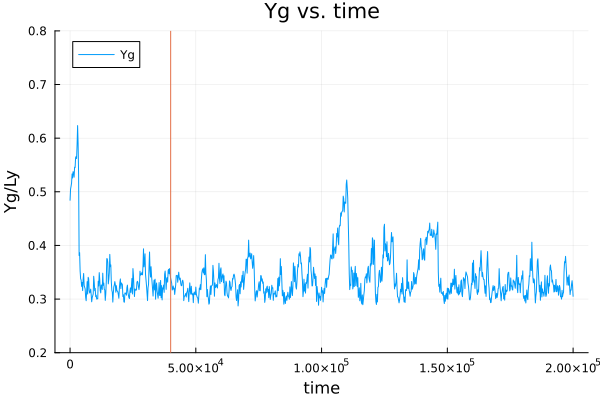
\includegraphics[width=\textwidth]{image/RaRtmap_time/2023-11-14T20:07:58.625__chi1.265_Ay50_rho0.4_T0.43_dT0.04_Rd0.0_Rt0.0_Ra0.938769_g0.0003999718779659611_run4.0e7_output.png}
      \subcaption{$\text{R}_\text{a}=0.938,\\\text{R}_\text{t}=0.0$}
      \label{}
    \end{minipage} &
    \begin{minipage}[t]{0.2\hsize}
      \centering
      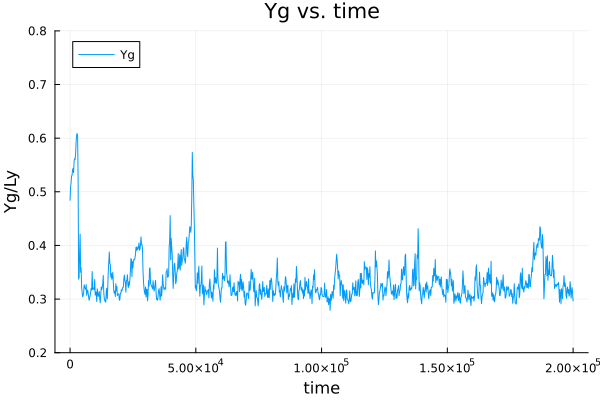
\includegraphics[width=\textwidth]{image/RaRtmap_time/2023-11-14T21:01:09.992__chi1.265_Ay50_rho0.4_T0.43_dT0.04_Rd0.0_Rt0.0_Ra1.4081535_g0.0003999718779659611_run4.0e7_output.png}
      \subcaption{$\text{R}_\text{a}=1.408,\\\text{R}_\text{t}=0.0$}
      \label{}
    \end{minipage} &
    \begin{minipage}[t]{0.2\hsize}
      \centering
      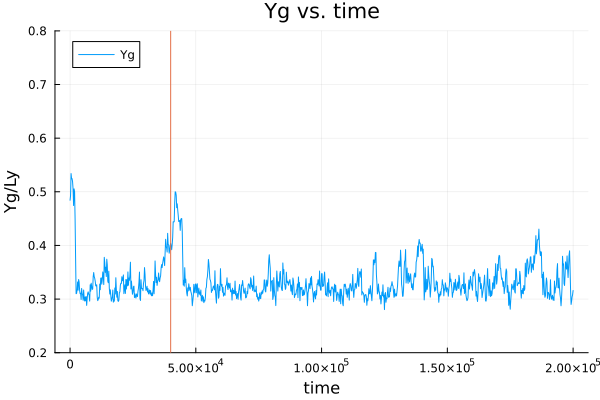
\includegraphics[width=\textwidth]{image/RaRtmap_time/2023-11-14T21:54:59.835__chi1.265_Ay50_rho0.4_T0.43_dT0.04_Rd0.0_Rt0.0_Ra1.877538_g0.0003999718779659611_run4.0e7_output.png}
      \subcaption{$\text{R}_\text{a}=1.877,\\\text{R}_\text{t}=0.0$}
      \label{}
    \end{minipage} \\
    \begin{minipage}[t]{0.2\hsize}
      \centering
      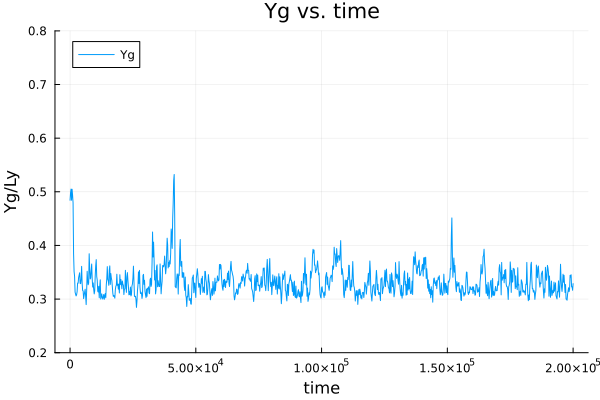
\includegraphics[width=\textwidth]{image/RaRtmap_time/2023-11-14T22:51:24.191__chi1.265_Ay50_rho0.4_T0.43_dT0.04_Rd0.0_Rt0.125_Ra0.0_g0.0003999718779659611_run4.0e7_output.png}
      \subcaption{$\text{R}_\text{a}=0.0,\\\text{R}_\text{t}=0.125$}
      \label{}
    \end{minipage} &
    \begin{minipage}[t]{0.2\hsize}
      \centering
      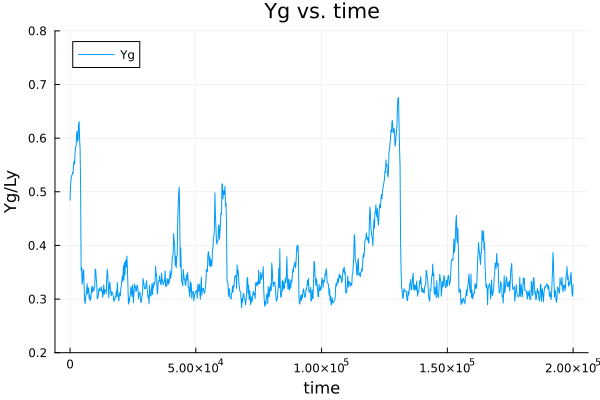
\includegraphics[width=\textwidth]{image/RaRtmap_time/2023-11-14T23:48:31.439__chi1.265_Ay50_rho0.4_T0.43_dT0.04_Rd0.0_Rt0.125_Ra0.4693845_g0.0003999718779659611_run4.0e7_output.png}
      \subcaption{$\text{R}_\text{a}=0.469,\\\text{R}_\text{t}=0.125$}
      \label{}
    \end{minipage} &
    \begin{minipage}[t]{0.2\hsize}
      \centering
      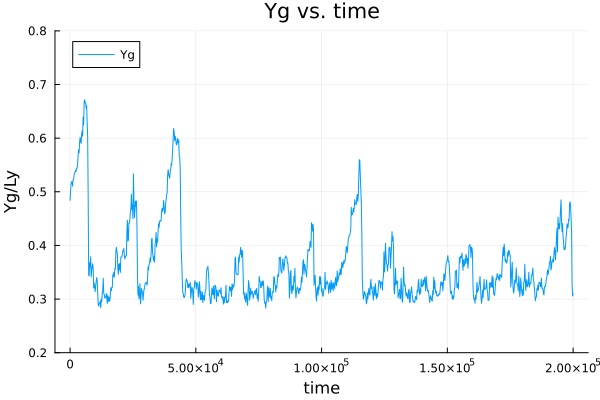
\includegraphics[width=\textwidth]{image/RaRtmap_time/2023-11-15T00:43:33.781__chi1.265_Ay50_rho0.4_T0.43_dT0.04_Rd0.0_Rt0.125_Ra0.938769_g0.0003999718779659611_run4.0e7_output.png}
      \subcaption{$\text{R}_\text{a}=0.938,\\\text{R}_\text{t}=0.125$}
      \label{}
    \end{minipage} &
    \begin{minipage}[t]{0.2\hsize}
      \centering
      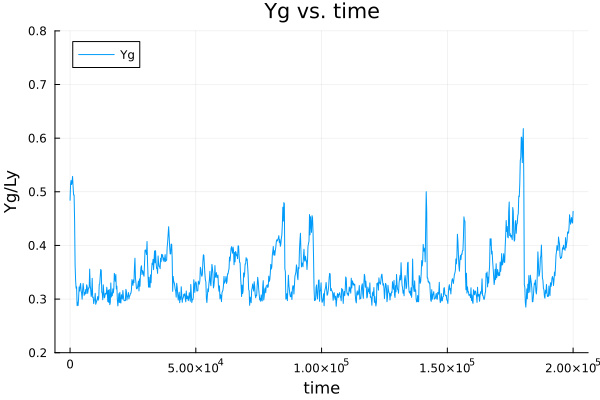
\includegraphics[width=\textwidth]{image/RaRtmap_time/2023-11-15T01:35:17.404__chi1.265_Ay50_rho0.4_T0.43_dT0.04_Rd0.0_Rt0.125_Ra1.4081535_g0.0003999718779659611_run4.0e7_output.png}
      \subcaption{$\text{R}_\text{a}=1.408,\\\text{R}_\text{t}=0.125$}
      \label{}
    \end{minipage} &
    \begin{minipage}[t]{0.2\hsize}
      \centering
      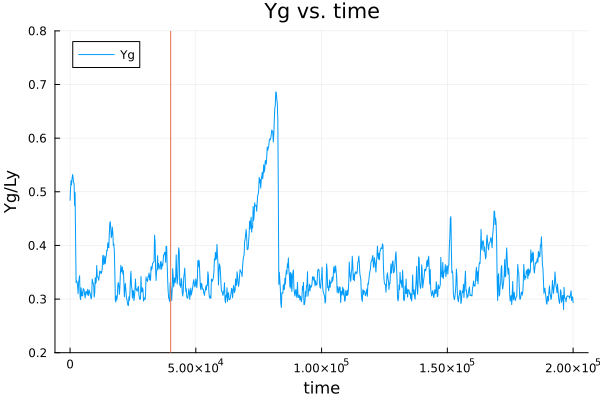
\includegraphics[width=\textwidth]{image/RaRtmap_time/2023-11-15T02:27:34.337__chi1.265_Ay50_rho0.4_T0.43_dT0.04_Rd0.0_Rt0.125_Ra1.877538_g0.0003999718779659611_run4.0e7_output.png}
      \subcaption{$\text{R}_\text{a}=1.877,\\\text{R}_\text{t}=0.125$}
      \label{}
    \end{minipage} \\
    \begin{minipage}[t]{0.2\hsize}
      \centering
      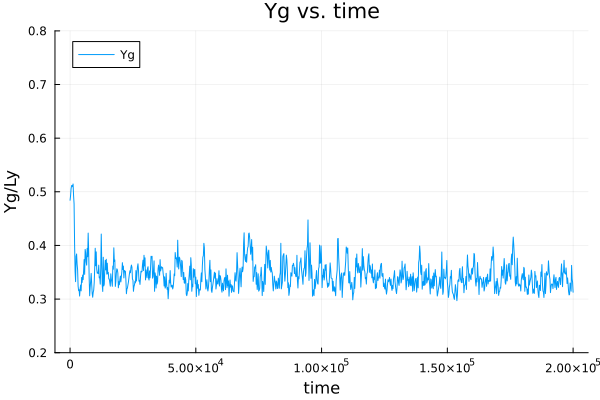
\includegraphics[width=\textwidth]{image/RaRtmap_time/2023-11-15T03:19:32.715__chi1.265_Ay50_rho0.4_T0.43_dT0.04_Rd0.0_Rt0.25_Ra0.0_g0.0003999718779659611_run4.0e7_output.png}
      \subcaption{$\text{R}_\text{a}=0.0,\\\text{R}_\text{t}=0.250$}
      \label{}
    \end{minipage} &
    \begin{minipage}[t]{0.2\hsize}
      \centering
      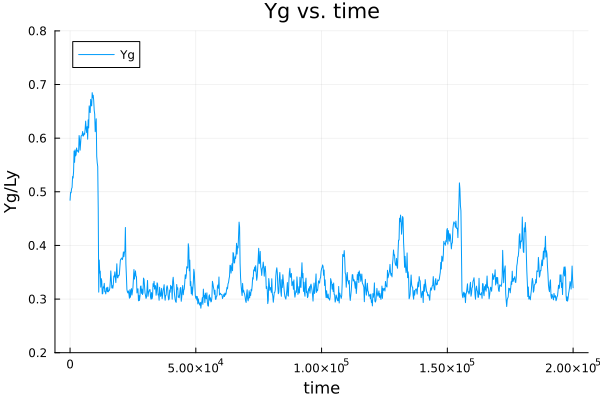
\includegraphics[width=\textwidth]{image/RaRtmap_time/2023-11-15T04:11:00.956__chi1.265_Ay50_rho0.4_T0.43_dT0.04_Rd0.0_Rt0.25_Ra0.4693845_g0.0003999718779659611_run4.0e7_output.png}
      \subcaption{$\text{R}_\text{a}=0.469,\\\text{R}_\text{t}=0.250$}
      \label{}
    \end{minipage} &
    \begin{minipage}[t]{0.2\hsize}
      \centering
      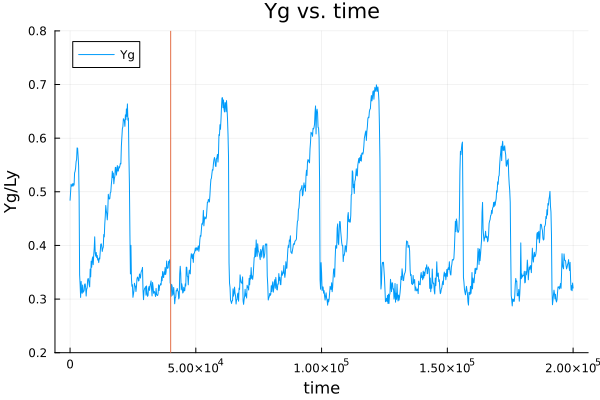
\includegraphics[width=\textwidth]{image/RaRtmap_time/2023-11-15T05:03:45.973__chi1.265_Ay50_rho0.4_T0.43_dT0.04_Rd0.0_Rt0.25_Ra0.938769_g0.0003999718779659611_run4.0e7_output.png}
      \subcaption{$\text{R}_\text{a}=0.938,\\\text{R}_\text{t}=0.250$}
      \label{}
    \end{minipage} &
    \begin{minipage}[t]{0.2\hsize}
      \centering
      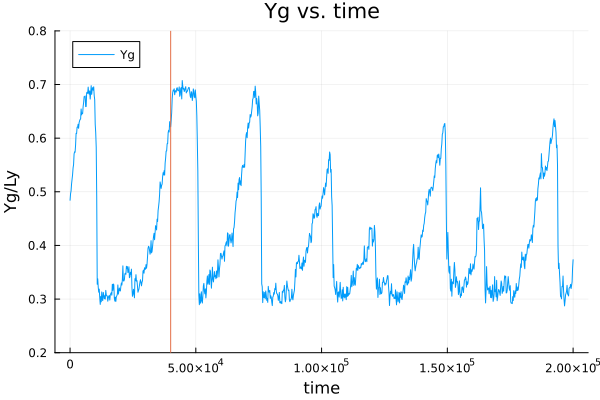
\includegraphics[width=\textwidth]{image/RaRtmap_time/2023-11-15T05:53:00.667__chi1.265_Ay50_rho0.4_T0.43_dT0.04_Rd0.0_Rt0.25_Ra1.4081535_g0.0003999718779659611_run4.0e7_output.png}
      \subcaption{$\text{R}_\text{a}=1.408,\\\text{R}_\text{t}=0.250$}
      \label{}
    \end{minipage} &
    \begin{minipage}[t]{0.2\hsize}
      \centering
      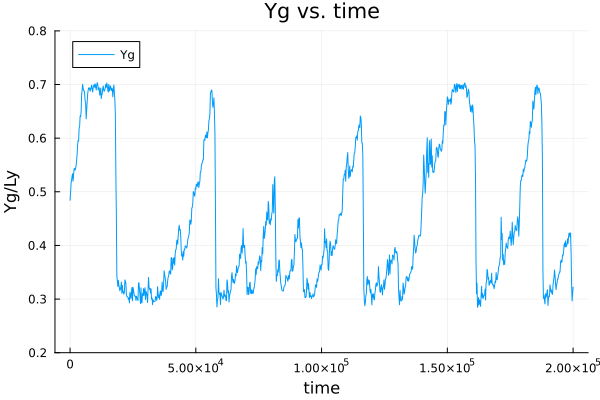
\includegraphics[width=\textwidth]{image/RaRtmap_time/2023-11-15T06:43:21.554__chi1.265_Ay50_rho0.4_T0.43_dT0.04_Rd0.0_Rt0.25_Ra1.877538_g0.0003999718779659611_run4.0e7_output.png}
      \subcaption{$\text{R}_\text{a}=1.877,\\\text{R}_\text{t}=0.250$}
      \label{}
    \end{minipage} \\
    \begin{minipage}[t]{0.2\hsize}
      \centering
      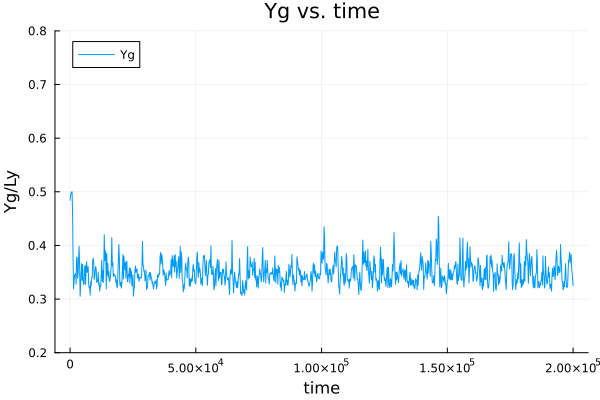
\includegraphics[width=\textwidth]{image/RaRtmap_time/2023-11-15T07:34:00.555__chi1.265_Ay50_rho0.4_T0.43_dT0.04_Rd0.0_Rt0.375_Ra0.0_g0.0003999718779659611_run4.0e7_output.png}
      \subcaption{$\text{R}_\text{a}=0.0,\\\text{R}_\text{t}=0.375$}
      \label{}
    \end{minipage} &
    \begin{minipage}[t]{0.2\hsize}
      \centering
      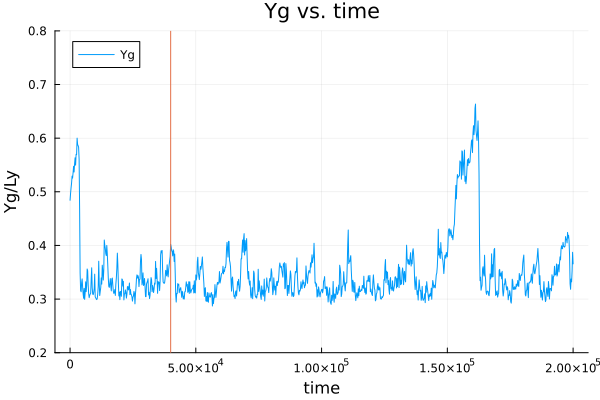
\includegraphics[width=\textwidth]{image/RaRtmap_time/2023-11-15T08:24:37.362__chi1.265_Ay50_rho0.4_T0.43_dT0.04_Rd0.0_Rt0.375_Ra0.4693845_g0.0003999718779659611_run4.0e7_output.png}
      \subcaption{$\text{R}_\text{a}=0.469,\\\text{R}_\text{t}=0.375$}
      \label{}
    \end{minipage} &
    \begin{minipage}[t]{0.2\hsize}
      \centering
      \includegraphics[width=\textwidth]{image/RaRtmap_time/2023-11-15T09:16:40.082__chi1.265_Ay50_rho0.4_T0.43_dT0.04_Rd0.0_Rt0.375_Ra0.938769_g0.0003999718779659611_run4.0e7_output.png}
      \subcaption{$\text{R}_\text{a}=0.938,\\\text{R}_\text{t}=0.375$}
      \label{}
    \end{minipage} &
    \begin{minipage}[t]{0.2\hsize}
      \centering
      \includegraphics[width=\textwidth]{image/RaRtmap_time/2023-11-15T10:07:20.945__chi1.265_Ay50_rho0.4_T0.43_dT0.04_Rd0.0_Rt0.375_Ra1.4081535_g0.0003999718779659611_run4.0e7_output.png}
      \subcaption{$\text{R}_\text{a}=1.408,\\\text{R}_\text{t}=0.375$}
      \label{}
    \end{minipage} &
    \begin{minipage}[t]{0.2\hsize}
      \centering
      \includegraphics[width=\textwidth]{image/RaRtmap_time/2023-11-15T10:59:30.665__chi1.265_Ay50_rho0.4_T0.43_dT0.04_Rd0.0_Rt0.375_Ra1.877538_g0.0003999718779659611_run4.0e7_output.png}
      \subcaption{$\text{R}_\text{a}=1.877,\\\text{R}_\text{t}=0.375$}
      \label{}
    \end{minipage} \\
    \begin{minipage}[t]{0.2\hsize}
      \centering
      \includegraphics[width=\textwidth]{image/RaRtmap_time/2023-11-15T11:53:37.697__chi1.265_Ay50_rho0.4_T0.43_dT0.04_Rd0.0_Rt0.5_Ra0.0_g0.0003999718779659611_run4.0e7_output.png}
      \subcaption{$\text{R}_\text{a}=0.0,\\\text{R}_\text{t}=0.500$}
      \label{}
    \end{minipage} &
    \begin{minipage}[t]{0.2\hsize}
      \centering
      \includegraphics[width=\textwidth]{image/RaRtmap_time/2023-11-15T12:45:26.303__chi1.265_Ay50_rho0.4_T0.43_dT0.04_Rd0.0_Rt0.5_Ra0.4693845_g0.0003999718779659611_run4.0e7_output.png}
      \subcaption{$\text{R}_\text{a}=0.469,\\\text{R}_\text{t}=0.500$}
      \label{fig:RaRtmap_time_Ra0.469_Rt0.500}
    \end{minipage} &
    \begin{minipage}[t]{0.2\hsize}
      \centering
      \includegraphics[width=\textwidth]{image/RaRtmap_time/2023-11-15T13:37:58.058__chi1.265_Ay50_rho0.4_T0.43_dT0.04_Rd0.0_Rt0.5_Ra0.938769_g0.0003999718779659611_run4.0e7_output.png}
      \subcaption{$\text{R}_\text{a}=0.938,\\\text{R}_\text{t}=0.500$}
      \label{fig:RaRtmap_time_Ra0.938_Rt0.500}
    \end{minipage} &
    \begin{minipage}[t]{0.2\hsize}
      \centering
      \includegraphics[width=\textwidth]{image/RaRtmap_time/2023-11-15T14:30:22.529__chi1.265_Ay50_rho0.4_T0.43_dT0.04_Rd0.0_Rt0.5_Ra1.4081535_g0.0003999718779659611_run4.0e7_output.png}
      \subcaption{$\text{R}_\text{a}=1.408,\\\text{R}_\text{t}=0.500$}
      \label{}
    \end{minipage} &
    \begin{minipage}[t]{0.2\hsize}
      \centering
      \includegraphics[width=\textwidth]{image/RaRtmap_time/2023-11-15T15:21:59.073__chi1.265_Ay50_rho0.4_T0.43_dT0.04_Rd0.0_Rt0.5_Ra1.877538_g0.0003999718779659611_run4.0e7_output.png}
      \subcaption{$\text{R}_\text{a}=1.877,\\\text{R}_\text{t}=0.500$}
      \label{}
    \end{minipage} 
  \end{tabular}
  \caption{$t_i = 0, t_f = 2.0 \times 10^5, \dd t \sqrt{\varepsilon / m \sigma^2}= 0.005, t \sqrt{\varepsilon / m \sigma^2} = 200 ごとにプロット.$}
  \label{fig:RaRtmap_time}
\end{figure}



\subsection{重力を先にかけて, 熱流を後からかける}

以下は, 追実験のときと同じように, まず重力のみをかけて, 粒子集団が落ちきってから熱流をかけると同時に測定を開始するものである.

\begin{figure}[H]
  \centering
  \includegraphics[scale=0.6]{image/RaRtmap_drop_time/2023-12-21T10:44:56.628_RaRtmap_chi1.265_Ay50_rho0.4_T0.43_dT0.04_Rd0.0_Rt0.0_Ra0.0_g0.0003999718779659611_run4.0e7.png}
  \label{}
  \caption{$\text{R}_\text{a}=0.0,\text{R}_\text{t}=0.0$}
\end{figure}

\begin{figure}[H]
  \begin{tabular}{ccccc}
    \begin{minipage}[t]{0.2\hsize}
      \centering
      \includegraphics[width=\textwidth]{image/RaRtmap_drop_time/2023-12-21T10:44:56.628_RaRtmap_chi1.265_Ay50_rho0.4_T0.43_dT0.04_Rd0.0_Rt0.0_Ra0.0_g0.0003999718779659611_run4.0e7.png}
      \subcaption{$\text{R}_\text{a}=0.0,\\\text{R}_\text{t}=0.0$}
      \label{fig:RaRtmap_drop_time_Ra0.0_Rt0.0}
    \end{minipage} &
    \begin{minipage}[t]{0.2\hsize}
      \centering
      \includegraphics[width=\textwidth]{image/RaRtmap_drop_time/2023-12-21T10:44:57.232_RaRtmap_chi1.265_Ay50_rho0.4_T0.43_dT0.04_Rd0.0_Rt0.0_Ra0.4693845_g0.0003999718779659611_run4.0e7.png}
      \subcaption{$\text{R}_\text{a}=0.469,\\\text{R}_\text{t}=0.0$}
      \label{}
    \end{minipage} &
    \begin{minipage}[t]{0.2\hsize}
      \centering
      \includegraphics[width=\textwidth]{image/RaRtmap_drop_time/2023-12-21T10:44:57.302_RaRtmap_chi1.265_Ay50_rho0.4_T0.43_dT0.04_Rd0.0_Rt0.0_Ra0.938769_g0.0003999718779659611_run4.0e7.png}
      \subcaption{$\text{R}_\text{a}=0.938,\\\text{R}_\text{t}=0.0$}
      \label{}
    \end{minipage} &
    \begin{minipage}[t]{0.2\hsize}
      \centering
      \includegraphics[width=\textwidth]{image/RaRtmap_drop_time/2023-12-21T10:44:57.379_RaRtmap_chi1.265_Ay50_rho0.4_T0.43_dT0.04_Rd0.0_Rt0.0_Ra1.4081535_g0.0003999718779659611_run4.0e7.png}
      \subcaption{$\text{R}_\text{a}=1.408,\\\text{R}_\text{t}=0.0$}
      \label{}
    \end{minipage} &
    \begin{minipage}[t]{0.2\hsize}
      \centering
      \includegraphics[width=\textwidth]{image/RaRtmap_drop_time/2023-12-21T10:44:57.455_RaRtmap_chi1.265_Ay50_rho0.4_T0.43_dT0.04_Rd0.0_Rt0.0_Ra1.877538_g0.0003999718779659611_run4.0e7.png}
      \subcaption{$\text{R}_\text{a}=1.877,\\\text{R}_\text{t}=0.0$}
      \label{}
    \end{minipage} \\
    \begin{minipage}[t]{0.2\hsize}
      \centering
      \includegraphics[width=\textwidth]{image/RaRtmap_drop_time/2023-12-21T10:44:57.529_RaRtmap_chi1.265_Ay50_rho0.4_T0.43_dT0.04_Rd0.0_Rt0.125_Ra0.0_g0.0003999718779659611_run4.0e7.png}
      \subcaption{$\text{R}_\text{a}=0.0,\\\text{R}_\text{t}=0.125$}
      \label{}
    \end{minipage} &
    \begin{minipage}[t]{0.2\hsize}
      \centering
      \includegraphics[width=\textwidth]{image/RaRtmap_drop_time/2023-12-21T10:44:57.600_RaRtmap_chi1.265_Ay50_rho0.4_T0.43_dT0.04_Rd0.0_Rt0.125_Ra0.4693845_g0.0003999718779659611_run4.0e7.png}
      \subcaption{$\text{R}_\text{a}=0.469,\\\text{R}_\text{t}=0.125$}
      \label{}
    \end{minipage} &
    \begin{minipage}[t]{0.2\hsize}
      \centering
      \includegraphics[width=\textwidth]{image/RaRtmap_drop_time/2023-12-21T10:44:57.672_RaRtmap_chi1.265_Ay50_rho0.4_T0.43_dT0.04_Rd0.0_Rt0.125_Ra0.938769_g0.0003999718779659611_run4.0e7.png}
      \subcaption{$\text{R}_\text{a}=0.938,\\\text{R}_\text{t}=0.125$}
      \label{}
    \end{minipage} &
    \begin{minipage}[t]{0.2\hsize}
      \centering
      \includegraphics[width=\textwidth]{image/RaRtmap_drop_time/2023-12-21T10:44:57.746_RaRtmap_chi1.265_Ay50_rho0.4_T0.43_dT0.04_Rd0.0_Rt0.125_Ra1.4081535_g0.0003999718779659611_run4.0e7.png}
      \subcaption{$\text{R}_\text{a}=1.408,\\\text{R}_\text{t}=0.125$}
      \label{}
    \end{minipage} &
    \begin{minipage}[t]{0.2\hsize}
      \centering
      \includegraphics[width=\textwidth]{image/RaRtmap_drop_time/2023-12-21T10:44:57.821_RaRtmap_chi1.265_Ay50_rho0.4_T0.43_dT0.04_Rd0.0_Rt0.125_Ra1.877538_g0.0003999718779659611_run4.0e7.png}
      \subcaption{$\text{R}_\text{a}=1.877,\\\text{R}_\text{t}=0.125$}
      \label{}
    \end{minipage} \\
    \begin{minipage}[t]{0.2\hsize}
      \centering
      \includegraphics[width=\textwidth]{image/RaRtmap_drop_time/2023-12-21T10:44:57.897_RaRtmap_chi1.265_Ay50_rho0.4_T0.43_dT0.04_Rd0.0_Rt0.25_Ra0.0_g0.0003999718779659611_run4.0e7.png}
      \subcaption{$\text{R}_\text{a}=0.0,\\\text{R}_\text{t}=0.250$}
      \label{}
    \end{minipage} &
    \begin{minipage}[t]{0.2\hsize}
      \centering
      \includegraphics[width=\textwidth]{image/RaRtmap_drop_time/2023-12-21T10:44:57.979_RaRtmap_chi1.265_Ay50_rho0.4_T0.43_dT0.04_Rd0.0_Rt0.25_Ra0.4693845_g0.0003999718779659611_run4.0e7.png}
      \subcaption{$\text{R}_\text{a}=0.469,\\\text{R}_\text{t}=0.250$}
      \label{}
    \end{minipage} &
    \begin{minipage}[t]{0.2\hsize}
      \centering
      \includegraphics[width=\textwidth]{image/RaRtmap_drop_time/2023-12-21T10:44:58.051_RaRtmap_chi1.265_Ay50_rho0.4_T0.43_dT0.04_Rd0.0_Rt0.25_Ra0.938769_g0.0003999718779659611_run4.0e7.png}
      \subcaption{$\text{R}_\text{a}=0.938,\\\text{R}_\text{t}=0.250$}
      \label{}
    \end{minipage} &
    \begin{minipage}[t]{0.2\hsize}
      \centering
      \includegraphics[width=\textwidth]{image/RaRtmap_drop_time/2023-12-21T10:44:58.129_RaRtmap_chi1.265_Ay50_rho0.4_T0.43_dT0.04_Rd0.0_Rt0.25_Ra1.4081535_g0.0003999718779659611_run4.0e7.png}
      \subcaption{$\text{R}_\text{a}=1.408,\\\text{R}_\text{t}=0.250$}
      \label{}
    \end{minipage} &
    \begin{minipage}[t]{0.2\hsize}
      \centering
      \includegraphics[width=\textwidth]{image/RaRtmap_drop_time/2023-12-21T10:44:58.197_RaRtmap_chi1.265_Ay50_rho0.4_T0.43_dT0.04_Rd0.0_Rt0.25_Ra1.877538_g0.0003999718779659611_run4.0e7.png}
      \subcaption{$\text{R}_\text{a}=1.877,\\\text{R}_\text{t}=0.250$}
      \label{}
    \end{minipage} \\
    \begin{minipage}[t]{0.2\hsize}
      \centering
      \includegraphics[width=\textwidth]{image/RaRtmap_drop_time/2023-12-21T10:44:58.258_RaRtmap_chi1.265_Ay50_rho0.4_T0.43_dT0.04_Rd0.0_Rt0.375_Ra0.0_g0.0003999718779659611_run4.0e7.png}
      \subcaption{$\text{R}_\text{a}=0.0,\\\text{R}_\text{t}=0.375$}
      \label{}
    \end{minipage} &
    \begin{minipage}[t]{0.2\hsize}
      \centering
      \includegraphics[width=\textwidth]{image/RaRtmap_drop_time/2023-12-21T10:44:58.322_RaRtmap_chi1.265_Ay50_rho0.4_T0.43_dT0.04_Rd0.0_Rt0.375_Ra0.4693845_g0.0003999718779659611_run4.0e7.png}
      \subcaption{$\text{R}_\text{a}=0.469,\\\text{R}_\text{t}=0.375$}
      \label{}
    \end{minipage} &
    \begin{minipage}[t]{0.2\hsize}
      \centering
      \includegraphics[width=\textwidth]{image/RaRtmap_drop_time/2023-12-21T10:44:58.387_RaRtmap_chi1.265_Ay50_rho0.4_T0.43_dT0.04_Rd0.0_Rt0.375_Ra0.938769_g0.0003999718779659611_run4.0e7.png}
      \subcaption{$\text{R}_\text{a}=0.938,\\\text{R}_\text{t}=0.375$}
      \label{}
    \end{minipage} &
    \begin{minipage}[t]{0.2\hsize}
      \centering
      \includegraphics[width=\textwidth]{image/RaRtmap_drop_time/2023-12-21T10:44:58.471_RaRtmap_chi1.265_Ay50_rho0.4_T0.43_dT0.04_Rd0.0_Rt0.375_Ra1.4081535_g0.0003999718779659611_run4.0e7.png}
      \subcaption{$\text{R}_\text{a}=1.408,\\\text{R}_\text{t}=0.375$}
      \label{}
    \end{minipage} &
    \begin{minipage}[t]{0.2\hsize}
      \centering
      \includegraphics[width=\textwidth]{image/RaRtmap_drop_time/2023-12-21T10:44:58.541_RaRtmap_chi1.265_Ay50_rho0.4_T0.43_dT0.04_Rd0.0_Rt0.375_Ra1.877538_g0.0003999718779659611_run4.0e7.png}
      \subcaption{$\text{R}_\text{a}=1.877,\\\text{R}_\text{t}=0.375$}
      \label{}
    \end{minipage} \\
    \begin{minipage}[t]{0.2\hsize}
      \centering
      \includegraphics[width=\textwidth]{image/RaRtmap_drop_time/2023-12-21T10:44:58.621_RaRtmap_chi1.265_Ay50_rho0.4_T0.43_dT0.04_Rd0.0_Rt0.5_Ra0.0_g0.0003999718779659611_run4.0e7.png}
      \subcaption{$\text{R}_\text{a}=0.0,\\\text{R}_\text{t}=0.500$}
      \label{}
    \end{minipage} &
    \begin{minipage}[t]{0.2\hsize}
      \centering
      \includegraphics[width=\textwidth]{image/RaRtmap_drop_time/2023-12-21T10:44:58.706_RaRtmap_chi1.265_Ay50_rho0.4_T0.43_dT0.04_Rd0.0_Rt0.5_Ra0.4693845_g0.0003999718779659611_run4.0e7.png}
      \subcaption{$\text{R}_\text{a}=0.469,\\\text{R}_\text{t}=0.500$}
      \label{fig:RaRtmap_drop_time_Ra0.469_Rt0.500}
    \end{minipage} &
    \begin{minipage}[t]{0.2\hsize}
      \centering
      \includegraphics[width=\textwidth]{image/RaRtmap_drop_time/2023-12-21T10:44:58.788_RaRtmap_chi1.265_Ay50_rho0.4_T0.43_dT0.04_Rd0.0_Rt0.5_Ra0.938769_g0.0003999718779659611_run4.0e7.png}
      \subcaption{$\text{R}_\text{a}=0.938,\\\text{R}_\text{t}=0.500$}
      \label{fig:RaRtmap_drop_time_Ra0.938_Rt0.500}
    \end{minipage} &
    \begin{minipage}[t]{0.2\hsize}
      \centering
      \includegraphics[width=\textwidth]{image/RaRtmap_drop_time/2023-12-21T10:44:58.872_RaRtmap_chi1.265_Ay50_rho0.4_T0.43_dT0.04_Rd0.0_Rt0.5_Ra1.4081535_g0.0003999718779659611_run4.0e7.png}
      \subcaption{$\text{R}_\text{a}=1.408,\\\text{R}_\text{t}=0.500$}
      \label{}
    \end{minipage} &
    \begin{minipage}[t]{0.2\hsize}
      \centering
      \includegraphics[width=\textwidth]{image/RaRtmap_drop_time/2023-12-21T10:44:58.955_RaRtmap_chi1.265_Ay50_rho0.4_T0.43_dT0.04_Rd0.0_Rt0.5_Ra1.877538_g0.0003999718779659611_run4.0e7.png}
      \subcaption{$\text{R}_\text{a}=1.877,\\\text{R}_\text{t}=0.500$}
      \label{}
    \end{minipage} 
  \end{tabular}
  \caption{$t_i = 2.4 \times 10^5, t_f = 4.0 \times 10^5, \dd t \sqrt{\varepsilon / m \sigma^2}= 0.005, t \sqrt{\varepsilon / m \sigma^2} = 200 ごとにプロット.$}
  \label{fig:RaRtmap_drop_time}
\end{figure}




\subsection{重力のみをかける}

\begin{itemize}
  \item $N = 1250$
  \item $\rho {\sigma}^2 = 0.4$
  \item $L_x / \sigma = 39.5\dots$
  \item $L_y / \sigma = 79.0\dots$
  \item $k_{\text{B}} T / \varepsilon = 0.43$
  \item $k_{\text{B}} \Delta T / \varepsilon = 0.0$
  \item $mg\sigma/\varepsilon = 4.0 \times 10^{-4}$
  \item $t_f \sqrt{\varepsilon / m \sigma^2} = 2.0 \times 10^{5}$
\end{itemize}

\subsection{熱流のみをかける}

\begin{itemize}
  \item $N = 1250$
  \item $\rho {\sigma}^2 = 0.4$
  \item $L_x / \sigma = 39.5\dots$
  \item $L_y / \sigma = 79.0\dots$
  \item $k_{\text{B}} T / \varepsilon = 0.43$
  \item $k_{\text{B}} \Delta T / \varepsilon = 0.04$
  \item $mg\sigma/\varepsilon = 0.0$
  \item $t_f \sqrt{\varepsilon / m \sigma^2} = 2.0 \times 10^{5}$
\end{itemize}


